\documentclass[twocolumn]{aastex62}

\usepackage{natbib}
\usepackage{amsmath}
\usepackage{amssymb}
\usepackage{amsfonts}
\usepackage{graphicx}
\usepackage{hyperref}
%\hypersetup{
%    colorlinks=true,
%    linkcolor=blue,
%    filecolor=magenta,      
%    urlcolor=cyan,
%}

\newcommand{\eps}{\ensuremath{\epsilon}}
\newcommand{\gam}{\ensuremath{\gamma}}
\newcommand{\Gam}{\ensuremath{\Gamma}}
\newcommand{\Del}{\ensuremath{\Delta}}

\newcommand{\gwbns}{GW170817A}
\newcommand{\grbbns}{GRB170817A}
\newcommand{\afterglowpy}{{\tt afterglowpy}}
\newcommand{\boxfit}{{\tt BoxFit}}
\newcommand{\python}{{\tt Python}}
\newcommand{\emcee}{{\tt emcee}}

\newcommand{\hubble}{{\em Hubble Space Telescope}}
\newcommand{\planck}{{\em Planck}}
\newcommand{\beppoSAX}{{\em BeppoSAX}}
\newcommand{\swift}{{\em Swift}}
\newcommand{\swiftXRT}{{\em Swift-XRT}}
\newcommand{\chandra}{{\em Chandra}}

\newcommand{\dd}{\ensuremath{\mathrm{d}}}
\newcommand{\Mej}{\ensuremath{M_{\mathrm{ej}}}}
\newcommand{\tobs}{\ensuremath{t_{\mathrm{obs}}}}
\newcommand{\tW}{\ensuremath{t_{\mathrm{w}}}}
\newcommand{\tb}{\ensuremath{t_{\mathrm{b}}}}
\newcommand{\tbm}{\ensuremath{t_{\mathrm{b-}}}}
\newcommand{\tbp}{\ensuremath{t_{\mathrm{b+}}}}
\newcommand{\tbpm}{\ensuremath{t_{\mathrm{b\pm}}}}
\newcommand{\tdec}{\ensuremath{t_{\mathrm{dec}}}}
\newcommand{\tumin}{\ensuremath{t_{\mathrm{min}}}}
\newcommand{\nuobs}{\ensuremath{\nu_{\mathrm{obs}}}}
\newcommand{\thobs}{\ensuremath{\theta_{\mathrm{obs}}}}
\newcommand{\phobs}{\ensuremath{\phi_{\mathrm{obs}}}}
\newcommand{\thW}{\ensuremath{\theta_{\mathrm{w}}}}
\newcommand{\thC}{\ensuremath{\theta_{\mathrm{c}}}}
\newcommand{\epse}{\ensuremath{\varepsilon_{\mathrm{e}}}}
\newcommand{\epseb}{\ensuremath{\bar{\varepsilon}_{\mathrm{e}}}}
\newcommand{\epsB}{\ensuremath{\varepsilon_{\mathrm{B}}}}
\newcommand{\sigT}{\ensuremath{\sigma_{\mathrm{T}}}}
\newcommand{\dL}{\ensuremath{d_{\mathrm{L}}}}
\newcommand{\qe}{\ensuremath{q_{\mathrm{e}}}}
\newcommand{\Mp}{\ensuremath{m_{\mathrm{p}}}}
\newcommand{\Me}{\ensuremath{m_{\mathrm{e}}}}
\newcommand{\Eiso}{\ensuremath{E_{\mathrm{iso}}}}
\newcommand{\Etot}{\ensuremath{E_{\mathrm{tot}}}}
\newcommand{\geff}{\ensuremath{g_{\mathrm{eff}}}}
\newcommand{\theff}{\ensuremath{\theta_{\mathrm{eff}}}}
\newcommand{\umin}{\ensuremath{u_{\mathrm{min}}}}
\newcommand{\umax}{\ensuremath{u_{\mathrm{max}}}}
\newcommand{\gmin}{\ensuremath{\gamma_{\mathrm{min}}}}
\newcommand{\gmax}{\ensuremath{\gamma_{\mathrm{max}}}}
\newcommand{\bmin}{\ensuremath{\beta_{\mathrm{min}}}}
\newcommand{\bmax}{\ensuremath{\beta_{\mathrm{max}}}}
\newcommand{\som}{\ensuremath{s_{\Omega}}}
\newcommand{\OO}{\ensuremath{\mathcal{O}}}


\begin{document}

\title{GRB Afterglows In The Multi-Messenger Era  OR  Electromagnetic Afterglows Of Structured Jets  OR  Structured Jets At All Angles}
\correspondingauthor{Geoffrey Ryan}
\email{gsryan@umd.edu}

\author[0000-0001-9068-7157]{Geoffrey Ryan}
\affil{Joint Space-Science Institute, University of Maryland, College Park, MD 20742, USA}

\author{Hendrik van Eerten}
\author{Luigi Piro}
\author{Eleonora Troja}


\begin{abstract}
	Gamma-ray bursts (GRBs) associated with gravitational wave events are, and will likely continue to be, viewed at a larger inclination than their fellow GRBs without gravitational wave detections.  As demonstrated by the afterglow of \gwbns{}, this requires an extension of the common GRB afterglow models which typically assume emission from an on-axis top hat jet.  We present a characterization of the afterglows arising from structured jets, utilizing both trans-relativistic numerical calculations and simple analytic approximations.  In many cases the temporal slope before the jet break is found to be a simple function of the ratio between the viewing angle and effective half opening angle of the jet.  This provides a useful handle in the analysis of structured GRB afterglow light curves, but does not completely resolve the degeneracy between viewing angle and jet structure model.  Our models, both numerical and analytic, are publicly available as the open source \python{} package \afterglowpy{}.
	
% Present new closure relations for structured jets, compare with established relations for choked jet models...	
	
	
\end{abstract}

\section{Introduction}

The binary neutron star merger event \gwbns{} provided, quite literally, a new view on gamma-ray burst (GRB) afterglows (CITE LIGO, Discovery papers).  Unlike typical short GRB afterglows, which begin bright and decay from detection with a ~week timescale, \gwbns{}'s non-thermal afterglow was undetectable for nine days whereupon it began steadily increasing in brightness in all bands for ~160 days \citep{Troja:2017aa, Troja:2018aa, van-Eerten:2018aa} (CITE OTHERS).  Very long baseline (VLBI) radio imagery over this period identified a radio core with an apparent superluminal motion, indicating the emitting surface was moving at relativistically at an oblique angle towards the Earth (CITE Mooley, Ghirlanda). The emission peaked at 160 days and proceeded to sharply decay at a rate commensurate with other short GRB afterglows (CITE YITL, peak-decay papers).

The lack of early emission, slow rising light curve, apparent motion of the radio centroid, and sharp decline post-peak are all consistent with emission from a \emph{structured jet}, a collimated blast wave with a non-trivial angular distribution of energy, viewed a moderate angle away from the jet axis (CITE YITL, Mooley, Ghirlanda, Lamb, Hotokezaka, ...).  The combined effects of a moderate viewing angle and angular structure in the jet produce a light curve significantly different from the standard on-axis uniform ``top-hat'' jet used extensively in GRB afterglow analysis. Since the gravitational wave signal of a binary neutron star merger is nearly isotropic, it is expected the majority of future GW-GRBs will also be viewed at significant inclination and may have similarly peculiar light curves as \gwbns{}.

A solid theoretical understanding of structured jet afterglows, including viewing angle effects, will be required to make the most use of future GW-GRB observations, the \gwbns{} dataset, and re-analysis of archival short GRBs.  To this end, we have calculated the explicit viewing angle and structure-dependent closure relations governing the afterglows of structured jets.  We have also developed the computational tool \afterglowpy{}: a public, open source \python{} package for on-the-fly computation of structured jet afterglows with arbitrary viewing angle.

Jet structure and viewing angle have a long history as potential explanations for temporal behaviors and breaks in GRB afterglows.  \citet{Meszaros:1998aa} first considered anisotropic models and noted they may present as ``orphan afterglows'' without a prompt GRB signal if viewed sufficiently off-axis.  Detailed theoretical calculations of structured jet afterglow light curves concluded several facts: on-axis structured light curves resemble those from top hat jets, off-axis structured light curves show a temporal break at an observer time $t_b$ that scales with the viewing angle $\thobs$ as $t_b\propto \thobs^{8/3}$, and the pre-break slope can depend on the viewing angle and particular structure model \citep{Rossi:2002aa, Dalal:2002aa, Granot:2002aa, Panaitescu:2003aa, Kumar:2003aa, Granot:2003aa, Salmonson:2003aa, Rossi:2004aa}. The ``Universal Structured Jet'' was a structured jet with isotropic-equivalent energy $E \propto \theta^{-2}$ proposed to explain the diversity of jet-break times as a viewing angle effect  \citep{Lipunov:2001aa, Zhang:2002aa}, although this was ultimately unsuccessful \citep{Nakar:2004aa}. 

The temporal break in the structured jet afterglow light curve can be more significant than in top hat models, and has been invoked to explain some observed jet breaks which do not easily fit the standard closure relations \citep{Panaitescu:2005aa, Panaitescu:2005ab}, although other dynamical and spectral processes can have similar effects (CITE Piro2005, COrsi\&Piro2006).  GRB prompt emission viewed significantly off-axis was (is?) the proposed origin for X-ray flashes \citep{Ioka:2001aa, Yamazaki:2002aa, Yamazaki:2003aa, Peng:2005aa}.  More recently, small non-zero viewing angles have been measured in a subset of the \swiftXRT{} afterglow sample \citep{Ryan:2015aa}.


In this paper, we calculate.  In Section \ref{sec:motivation} we review the general properties of structured jets and their necessity to GRB afterglows.  In Section \ref{sec:numerical} we develop our theoretical framework and describe its numerical implementation in \afterglowpy{}.  Section \ref{sec:structuredJets} characterizes the general behavior of structured jet afterglow light curves, provides the closure relations with explicit viewing angle dependence, and relates structured jets to standard energy injection models.  Section \ref{sec:gw170817} demonstrates an application to \gwbns{}. Section \ref{sec:discussion} gives further discussion and Section \ref{sec:summary} gives the summary.  Detailed derivation of the closure relations is provided in Appendices \ref{app:derive1} and \ref{app:derive2}.


\newpage

\subsection{Old Draft}

The binary neutron star merger \gwbns{} and its associated electromagnetic counterparts provided a wealth of data to high energy astrophysics (CITE).  Not least among these was its peculiar non-thermal afterglow, first detected in X-rays 9 days after the merger \citep{Troja:2017aa}.  This was followed by radio 16 days after the merger and optical 73 days after the merger (CITE Radio \& Optical follow-up).  Unlike any short gamma-ray burst (GRB) afterglow observed before, \grbbns{} steadily {\em rose} in brightness for ~160 days in all observed bands.  After peak, the emission quickly decayed at a rate similar to other GRB afterglows.

The absence of early X-ray emission, with early non-detections by \swiftXRT{} and a deep upper limit from \chandra{}, led early analyses to consider the effect if viewing angle on the emission \citep{Troja:2017aa} (CITE MORE).  Given the gravitational wave signal of a binary neutron star merger is observable almost regardless of of orientation, it is in fact expected that GRB/GW events would be viewed at moderate inclination.

As \grbbns{}'s afterglow continued to rise for weeks after the burst, it became evident the emission could not be explained by a simple uniform ``top hat'' jet viewed off axis.  More sophisticated models were considered: ``structured jets'' with non-uniform angular distribution of energy and quasi-isotropic ``refreshed shocks'' with significant velocity stratification of the ejecta and modest Lorentz factors.  The observation of apparent superluminal motion of the radio centroid and the steep turnover of the light curve after 160 days confirmed the relativistic and collimated nature of the outflow, in accordance with the structured jet picture (CITE Mooley, Ghirlanda, YITL, other steepening paper).

It is expected, of course, that 

Structured jets, blast waves with a non-uniform angular distribution of energy, have been invoked to explain several temporal features in GRB afterglow light curves.  

\subsubsection{History of structure and viewing angle}

The first GRB afterglow was discovered by \beppoSAX{} as part of GRB 970228 \citep{Wijers:1997aa}.  GRB afterglows present as broadband synchrotron emission following the prompt gamma-ray signal and can last for days, weeks, months, and years.  


\subsubsection{What we're doing}

In this paper we develop a theoretical model of the electromagnetic afterglow of generic structured jets for arbitrary viewing inclinations.  The model takes as input the energy and Lorentz factor angular profiles, which may be intrinsic to the jet launching mechanism 

The light curves resemble broken power laws.  We calculate viewing angle dependent closure relations, directly relating the effective temporal evolution of the light curve to the viewing angle and explosion geometry.  



\newpage

\subsection{Lit Review}
\begin{itemize}
\item \citet{Meszaros:1998aa} First discusses effect of angular structure in $E$ and $\Gamma$, predicts rising light curves when seen off axis, calculates closure relations in various cases.
\item \citet{Nakamura:1999aa} Far off-axis emission from top-hat jet in stellar wind environment, application to GRB 980425.
\item \citet{Moderski:2000aa} Relativistic effects (equal arrival time surface, etc) smear jet-break.
\item \citet{Ioka:2001aa} Viewing angle dependent prompt emission.  GRB prompt peak $L$ - spectral lag relation from viewing angle.  
\item \citet{Lipunov:2001aa, Zhang:2002aa} universal structured jet, $\theta^{-2}$, may explain jet breaks, etc.
\item \citet{Rossi:2002aa} Considers jets with $E\propto \theta^{-2}$.  Verifies at early times line-of-sight material dominates over core and wings, light curves resemble on-axis top-hats, but jet break is due to observer angle.  Simple emission model.  Postulates variety of jet-breaks due to off-axis structured jets, instead of distribution of $\Eiso$, $\thC$.  $t_b \propto \thobs^{8/3}$.  
\item \citet{Dalal:2002aa} Considers emission from boosted lightbulb, refers to $\thobs > \theta_j$ as ``off-axis,'' points out off-axis jet breaks will be delayed and dim, light curves converge at late time.
\item \citet{Granot:2002ab} Off-axis viewing of top hat jets, computed as boosted light bulb, analytic top-hat, and hydro sim. $\thobs < \theta_j$ look like on-axis top-hats, jet breaks increase with $\thobs$, evidence for $\thobs$-dependent slope before jet break in hydro models.
\item \citet{Yamazaki:2002aa, Yamazaki:2003aa} XRF as off-axis prompt GRB using \citet{Ioka:2001aa} model.
\item \citet{Panaitescu:2003aa} Off-axis viewing of power-law jets $E\propto \theta^{-q}$ with sharp cores.  Analytic blast waves, detailed treatment of relativistic emission and synchrotron spectrum. When viewing within the core, no large effect so long as $q \geq 2$.  Analytic formulae for aligned observers, numerical only for misaligned.  Core visible at $t_a \sim E_0^{1/3} \thobs^{8/3}$ in ISM.  Structure may only steepen jet breaks, proposes examining pre- and post- jet break slopes to determine whether structure is evident.
\item \citet{Kumar:2003aa} Numerical evolution of radially-integrated Gaussian, top-hat, and power-law jets/  ``Therefore, a simple model in which the energy per unit solid angle is taken to be time independent and each element of the jet behaves as if it were part of a spherical flow with the same can serve as a useful approximation for the jet dynamics, as long as the jet is sufficiently relativistic.''
\item \citet{Granot:2003aa} ``structured jet:'' jet with angular structure. Smooth power law in $\Theta = \sqrt{1 + \theta^2/\thC^2}$.  Analysis of power-law jet light curves from \citet{Kumar:2003aa}. Only considers USJ, top-hat, and permutations.  Find deviations from top-hat appearance small, USJ must have $E\approx \theta^{-2}$, $\Gamma\approx \theta^{0 < 1}$.
\item \citet{Salmonson:2003aa} Numerical and analytic study of top-hat and structured jets.  Computes doppler factor and angular size in asymptotic limits (no cooling frequency), finds far-off-axis closure relations.  Examines `bump' seen when initially strongly beamed emission becomes structured, then proceeds to jet break.
\item \citet{Nakar:2004aa} Distribution of luminosity and jet-breaks rules out USJ. 
\item \citet{Rossi:2004aa}. Light curves and polarization for top-hat, USJ, and Gaussian jet.  Gaussian jet shows slowly rising flux at sufficiently large viewing angles. Time dependence of polarization signal may distinguish between USJ and Gaussian.
\item \citet{Yamazaki:2004aa} $E_P$ -- $E_{iso}$ prompt relation from viewing angle.
\item \citet{Peng:2005aa} Two-component (narrow + wide) jet, afterglows, blurred jet breaks, off-axis as XRF.
\end{itemize}

\subsection{Old Old Draft}

The electromagnetic afterglow of \gwbns{} gave, quite literally, a new view on gamma-ray burst (GRB) afterglows.  

A canonical afterglow was almost immediately ruled out \citep{Troja:2017aa}.  


The structure of the blast wave giving rise to gamma-ray burst (GRB) afterglows has been a subject of interest since their discovery by \beppoSAX{} in GRB 970228 \citep{Wijers:1997aa}.

{\color{blue} LUIGI: ?was found since early afterglow observations with BeppoSAX, when the
presence of a structured outflow has been considered for explaining some of the
temporal breaks observed in the light curves of a number of GRBs (Panaitescu and
Kumar 2003, Apj 592: 390, Panaitescu 2005 MNRAS 362, 921). Candidates for
structured jet exhibit a variation of the decay index at the break smaller that that
expected for a top-hat spreading jet ($\Delta \alpha \approx 0.8$) and larger than
that induced by the crossing of the cooling frequency ($\Delta\alpha=0.25$). Energy
injection by a long lasting central engine can also induce temporal breaks, either
flattening or steepening. Other effects such as transition to non-relativistic
expansion, the transition from wind-like to ISM (Piro et al. 2005, Apj 623 314) or the
emergence of an Inverse compton component (Corsi \& Piro
2006A\&A...458..741C) can also produce breaks, in these case associated with a
flattening of the light curve.
More recenlty Ryan et al (2015) presented evidence of a structured jet in a sample
based on SWIFT observations. Considering the number of processes that can
produce breaks mentioned above, no undisputable observational evidence of a
structured jet became available till the observations of GW170817. Real jets}


Gamma-ray burst (GRB) afterglows, since their discovery by \beppoSAX{} in GRB 970228, have been a potent tool for studying GRBs and their progenitors.



Gamma-ray burst (GRB) afterglows are commonly modeled as top hat blast waves with no internal structure pointed directly at the observer. This has been largely sufficient given the available data, although some evidence of viewing angle effects has been found \citep{Ryan:2015aa}.  New observational capabilities have witnessed new phases of afterglow evolution, such as the discovery of plateaus with Swift.  Real jets (of course) have internal structure, but the top hat assumption has been a sufficiently spherical cow. 

\gwbns{} changes the picture: new object with a strange afterglow.  Steep/late rise, LONG slow rise, turnover at 160d.  The slow rise is impossible to reproduce with standard afterglow evolution: first observation of a \emph{structured} phase of evolution. 

The dominant contribution may be an angular distribution of energy within the blast wave (``structured jet'') combined with off-axis viewing (CITE Rossi04).  For \gwbns{} this corresponds to the ``successful jet'' picture.  Alternately, radial stratification of velocity (``refreshed shock'') can cause a similar phase, most simply with a quasi-spherical (or at least top-hat) angular structure.  This situation is produced by the ``choked jet''  or ``cocoon'' picture of \gwbns{}. Understanding the effects of both structures on afterglows, and their dependence on the parameters of the burst, are vital to understanding GW counterparts.

To this end, we have calculated the power law temporal slope of the structured phase in both angular and radial structure dominated cases, along with the corresponding observed break times.  We have developed a semi-analytic numerical model of structured GRB afterglows for detailed comparison to data, which is now publicly available.

Summary: In section 2 we discuss structured jets, in section 3 refreshed shocks, in section 4 our numerical model, section 5 application to \gwbns{}, and section 6 future applications and discussion.

\section{Motivation: Why Structured Jets?}\label{sec:motivation}

The \emph{structured jet} is a GRB emission model where the isotropic-equivalent energy of a blast wave is a function of the angle from the jet axis: $\Eiso = E(\theta)$. The specific structure of a jet is determined by the intrinsic structure of the jet launching mechanism as well as the sculpting that occurs as the jet burrows out of the encasing ejecta debris (as in a binary neutron star merger) or stellar envelope (as in a collapsar).  

Numerical simulations have revealed a variety of jet angular energy distributions, often containing an energetic core with power law tails.  Figure \ref{fig:jetStruct} shows a collection of jet energy distributions from the literature \citep{Aloy:2005aa, Mizuta:2009aa, Duffell:2013aa, Lazzati:2017aa, Margutti:2018aa}.  Lacking a well-established physical model of the true $E(\theta)$, in particular its dependence on the parameters of the system, we consider two simple parameterized models: a Gaussian jet and a power law jet with a smooth core.  

\begin{align}
	E(\theta) &= E_0 \exp\left(-\frac{\theta^2}{2\thC^2}\right)  && \text{Gaussian} \label{eq:gauss}\\
	E(\theta) &= E_0 \left(1 + \frac{\theta^2}{b\thC^2} \right)^{-b/2}  && \text{power law} \label{eq:pl}
\end{align}

%
% Update jet Structure models paper.
%

\begin{figure}
	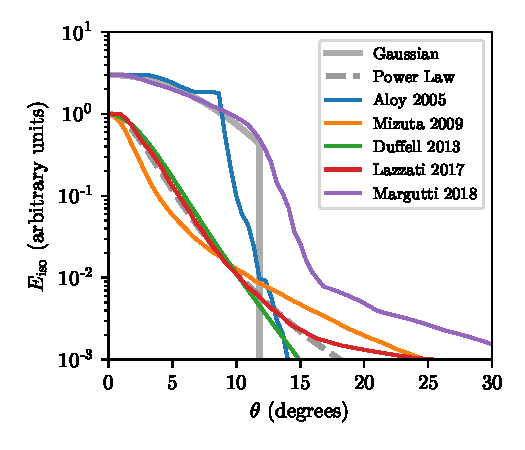
\includegraphics[width=\columnwidth]{figs/jetStructureComparison.pdf}
	\caption{Lateral profiles of isotropic equivalent energy $\Eiso$ as a function of angle from the jet axis $\theta$, individually rescaled to group similar profile shapes.  The thick grey lines show fiducial profiles with simple analytic expressions (Equations \eqref{eq:gauss} and \eqref{eq:pl}) while the thin colored lines show results from numerical simulations and analytic models chosen from the literature.  The blue line is the B1 numerical simulation of \cite{Aloy:2005aa}, orange the HE16N numerical simulation of \cite{Mizuta:2009aa}, green an analytic ``boosted fireball'' model with $\gamma_{\rm{B}}=10$ and $\eta_0=3$ from \cite{Duffell:2013aa}, red the numerical simulation from \cite{Lazzati:2017aa} (L17), and purple the numerical simulation from \cite{Margutti:2018aa} (M18).  The thick solid grey line is a Gaussian profile (Equation \eqref{eq:gauss}) with $E_0 = 3\times 10^{52}$ erg, $\thC = 6^\circ$, and $\thW=12^\circ$ and the thick dashed grey line is a smoothed power law profile (Equation \eqref{eq:pl}) with $E_0 = 10^{52}$ erg, $\thC = 2^\circ$, $\thW=20^\circ$, and $b=4.5$.  The Gaussian and power law profiles can emulate the basic properties of the energy profiles found in the literature. \label{fig:jetStruct}}
\end{figure}

Each fiducial model is parameterized by a normalization $E_0$, a width $\thC$, and a truncation angle $\thW$.  The power law model also retains a power law index $b$.  Outside $\thW$ the energy is initially zero, this acts as an outer truncation angle for the jet.   Our power law profile includes a factor of $b^{-1}$ in the base which does not usually appear in the literature \citep{Granot:2003aa, Hotokezaka:2018aa}.  This serves to normalize the value of $\thC$ and make it comparable between power laws of different $b$ and Gaussian jets.  Both structure profiles obey
\begin{equation}
	\left . \frac{d^2}{d\theta^2} \log E \right \rvert_{\theta=0} = -\frac{1}{\thC^2}\ , \label{eq:thCdef}
\end{equation} 
which we take as a generic definition for $\thC$.

Figure \ref{fig:jetStruct} shows an example of each model together with jet energy profiles drawn from the literature, mostly the result of numerical relativistic hydrodynamic simulations.  The Gaussian profile emulates jets with a flat core and sharp edges, typically the result of powerful successful jets \citep{Aloy:2005aa, Margutti:2018aa}.  Jets which are subject to stronger interactions with the surrounding medium can develop a profile with energetic wings and a narrow core, emulated by the analytic power law profile \citep{Mizuta:2009aa, Duffell:2013aa, Lazzati:2017aa}.  

A generic energy profile $E(\theta)$, for instance from a numerical hydrodynamics simulation, may have several more parameters, but one can still associate with it an on-axis energy $E_0 = E(0)$ and an effective core width $\thC \sim |E''(0)/E_0|^{-1/2}$ which should fully specify the leading order near on-axis behaviour.  

The afterglow light curve of a structured jet follows one of two qualitatively different regimes depending on the orientation of the viewer with respect to $\thC$.  We refer to the regimes as ``aligned'' when $\thobs < \thC$, and ``misaligned'' when $\thobs > \thC$.  



\section{Methods And The \afterglowpy{} Package}\label{sec:numerical}

To compute the light curves of structured jet afterglows we constructed numerical and analytic models utilizing the single shell approximation of \cite{van-Eerten:2010aa, van-Eerten:2018ab}.  This approach integrates over the massive ejecta, contact discontinuity, and forward shock complex, treating it as a single fluid element with uniform radial structure. We utilize a trans-relativistic equation of state which smoothly interpolates between the ultra-relativistic and non-relativistic limits and include an approximate prescription for jet spreading.  This approach, with a simplified equation of state and jet spreading model, has been used successfully to model the synthetic light curves of top hat jets from multidimensional numerical relativistic hydrodynamics simulations \citep{van-Eerten:2010aa}.

In the ultra-relativistic limit the single shell approximation provides useful scaling relations to compute the structured jet closure relations presented in Section \ref{sec:structuredJets}.  The full trans-relativistic numerical model is publicly available as the \afterglowpy{} Python package, described in more detail in Section \ref{subsec:afterglowpy}.

We utilize a standard spherical coordinate system $(r, \theta, \phi)$ with origin at the GRB central engine and polar axis aligned with the jet axis.  The blast wave forward shock has a radial position $R(t, \theta)$, where $t$ is the time measured in the burster frame. The observer is located in a direction $\hat{\bf n}$ which makes an angle $\thobs$ with the $z$-axis, $\hat{\bf n} \cdot \hat{\bf z} = \cos \thobs$, and is oriented along the $x$-axis, $\phobs = 0$.  A particular point on the blast wave $\hat{\bf r} = (\theta, \phi)$ makes an angle $\psi$ (with cosine $\mu$) with the viewer, $\mu = \cos \psi = \hat{\bf n} \cdot \hat{\bf r}$.

\subsection{The Single Shell Approximation}\label{subsec:algo}

The observed flux $F_\nu(\tobs, \nuobs)$ at observer time $\tobs$ and frequency $\nuobs$ is calculated via:
\begin{equation}
	F_\nu(\tobs, \nuobs) = \frac{1+z}{4\pi \dL^2} \int \! \dd \Omega\  \dd r\ r^2 \delta^2\ \epsilon'_{\nu'} \ , \label{eq:flux}
\end{equation}
where $z$ is the redshift of the source, $\dL$ is the luminosity distance, $\delta$ the doppler factor of the emitting fluid with respect to the observer, and $\epsilon'_{\nu'}$ the fluid rest-frame emissivity.

To accommodate an initial structure profile $E(\theta)$ we consider the integrand of Equation \eqref{eq:flux} as a function of the polar angle $\theta$.  We assume each constant-$\theta$ annulus evolves independently, as an equivalent top hat of initial width $\theta_j = \theta$.  This is a very good approximation when transverse velocities are low: when the blast wave is ultra-relativistic and has not begun to spread and when the blast wave is non-relativistic and the spreading has ceased \citep{van-Eerten:2010aa}.  Once jet spreading begins in earnest the errors are larger, and this approach can be best viewed as an interpolation between the correct ultra-relativistic and non-relativistic limits \citep{van-Eerten:2010aa}.
 
To compute the light curve of a top-hat jet of initial width $\thC$ we first must calculate the time evolution of the blast wave. In the single-shell approximation we treat the ejecta mass, contact discontinuity, and forward shock as a single unit propagating through a cold ambient medium with constant rest-mass density $\rho_0 = \Mp n_0$.  We utilize the TM trans-relativistic equation of state to describe the fluid consistently throughout its evolution \citep{Mignone:2005aa}.  The forward shock is a radius $R$ from the explosion, and the fluid behind the shock has four-velocity $u$ and Lorentz factor $\gamma$.  The shock jump conditions can be used to determine the shock speed:
\begin{equation}
	\dot{R} = \frac{4 u \gamma}{4 u^2 +3}c\ . \label{eq:Rdot}
\end{equation}
Here the time derivative $\dot{R}$ is taken with respect to elapsed time in the bursters' frame $t$.  

 The evolution of the four velocity is determined through conservation of energy.  The total energy in the trans-relativistic single shell approximation is:
\begin{align}
	E &= (\gamma - 1)\Mej c^2 + \frac{4\pi}{9} \rho_0 c^2 R^3 (4 u^2 + 3) \beta^2 f_\Omega \ , \label{eq:E} \\
	f_\Omega &= 2 \sin^2\left( \theta_j / 2 \right)\ . \label{eq:fOm}
\end{align}
In Equation \eqref{eq:E} the first term is the kinetic energy of the ejected mass $\Mej$, assumed to have already accelerated and adiabatically cooled to its coasting velocity. The second term is the kinetic and thermal energy of the shocked ISM with three-velocity $\beta = u / \gamma$.  Equation \eqref{eq:fOm} describes the fractional solid angle of the jet in terms of the time dependent opening angle $\theta_j(t)$. While the blast wave is relativistic $\theta_j = \thC$ and $f_\Omega$ is constant, but once the jet edge comes in causal contact with the core it begins to spread due to its own internal pressure. The jet spreads and $\theta_j$ increases until the blast wave is spherical and $f_\Omega=1$.  The spreading occurs at sound speed $c_s$ in the fluid rest-frame, causing the opening angle of the jet to increase as \citep{van-Eerten:2010aa, Duffell:2018aa}:
\begin{equation}
	\dot{\theta_j} = \frac{c_s}{\gamma R}\ , \qquad \text{if } u < 1/3\thC \text{ and } \theta_j > \pi/2\ . \label{eq:thetadot}
\end{equation}
The criterion $u < 1/3\thC$ is satisfied when a sound wave can propagate from $\theta = \thC$ to $\theta=0$ in a blast wave propagating in a uniform ISM (CITE HENDRIK).  It is similar to the condition given in \cite{Duffell:2018aa}, which found a numerical factor of 2.5 (instead of 3) after calibrating to numerical simulations.  Our criteria differs from that used in \citet{Troja:2018aa, Piro:2019aa, van-Eerten:2018aa} which used an overly simplistic $u < 1$ criterion to begin jet spreading.

Given an expression for $E$ in terms of $t$, $R$, $u$, and $\theta_j$, Equation \eqref{eq:E} may be differentiated with respect to $t$ and solved for $\dot{u}$. A standard adiabatic evolution will maintain $E=$ constant, while in a continuously refreshed shock scenario $E = E_{>u}(u)$ and in standard energy injection models $E \propto t^-q$.  This defines a three dimensional system of ordinary differential equations (ODEs) in the variables $(R, u, \theta_j)$ which may be solved numerically or, in certain limits, analytically from appropriate initial conditions.

Once the shock evolution ($R(t)$, $u(t)$, $\theta_j(t)$) is known, the flux is given by the integral:
\begin{align}
	F_\nu(\tobs, \nuobs) &= \frac{1+z}{4\pi \dL^2} \int \! \dd \Omega\ R^2\ \Delta R\  \delta^2\ \epsilon'_{\nu'} \ , \label{eq:flux2}
\end{align}
where $\Delta R$ is the effective shock width contributing to the emission \citep{van-Eerten:2010aa}:
\begin{equation}
	\Delta R = \frac{1}{1-\mu \dot{R}} \frac{R}{12\gamma^2} \ . \label{eq:dr}
\end{equation}
 The integrand is evaluated at a constant observer time $\tobs$ and observer frequency $\nuobs$, related to $t$ and $\nu'$ by:
\begin{align}
	\tobs &= (1+z) \left(t - \mu(\theta, \phi) R(t)/c\right)\ , \label{eq:tobs} \\
	\nuobs &= (1+z)^{-1} \delta \nu' , \label{eq:nuobs}
\end{align}

The rest-frame synchrotron emissivity may be calculated to numerous ways with varying degrees of physics and accuracy.  We use the standard broken power law formalism with characteristic frequencies $\nu_m$ and $\nu_c$, with the cooling frequency $\nu_c$ calculated via the global cooling approximation \citep{Granot:2002aa, van-Eerten:2010aa}.


\subsection{\afterglowpy{}} \label{subsec:afterglowpy}


We have constructed the \afterglowpy{} Python package to implement the numerical computation of light curves according to Section \ref{subsec:algo} and provide it to the community.  The integration routine itself is written in C, wrapped as an extension for Python, and has been optimized to be used in intensive data analysis routines such as Markov Chain Monte-carlo which can require many thousands or millions of evaluations.  

\afterglowpy{} uses a standard RK4 algorithm to evolve the $(R(t), u(t), \theta_j(t))$ system of equations on a fixed logarithmically spaced grid of $t$.  The endpoints of the $t$-grid are chosen to bracket the burster frame times required to calculate the requested $\tobs$.  Initial conditions for $R$, $u$, and $\theta$ are typically those of a decelerating ultra-relativistic blast wave.  The user can set the density of the $t$-grid with the {\tt tRes} parameter: the number of grid points per decade of $t$.  The default value for {\tt tRes} is 1000, which is sufficiently dense that the shock ODE evolution is not the dominant error source but not so dense as to adversely impact performance.

Each top-hat jet component is integrated in $\theta$ and $\phi$ using an adaptive Romberg scheme with a fixed relative tolerance of $10^{-6}$ and an adaptive absolute tolerance.  When summing over top-hat components of a structured jet, the innermost (core) component is calculated first.  As the calculation proceeds, the current running sum of the flux is used to set absolute tolerance for the next component.  This minimizes the computations performed on dim, off-axis sectors of the jet.  

Each evaluation of the integrand requires a binary search to determine the burster time $t$ at which to evaluate $R$, $u$, and $\theta_j$.  Fluid quantities are then calculated using the shock-jump conditions and the synchrotron emissivity is evaluated using the standard external shock formulae \citep{Granot:2002aa,van-Eerten:2010aa}.  

The numerical accuracy of a top-hat light curve with this integration scheme is typically better than $10^{-4}$.  The structured jet calculation splits the integration domain into {\tt latRes} disjoint annuli, each evolved as an independent top-hat and their emission summed.  By default {\tt latRes} is chosen such that there will be 5 zones per $\thC$-sized interval of $\theta$.   The choice of  {\tt latRes} has the largest impact on the code performance and accuracy.  We find the choice $\mathtt{latRes} = 5$ gives sufficiently quick performance at acceptable errors, typically on the order of $10^{-2}$.  TODO SHOW CONVERGENCE PLOT


\subsection{Comparison To \boxfit{}} \label{subsec:boxfitcomp}

\afterglowpy{}, in utilizing the semi-analytic methods of Section \ref{subsec:algo}, trades some amount of physical accuracy for great flexibility.  We gauge this trade-off by comparing to the \boxfit{} code, a standard tool which calculates high fidelity afterglow light curves based on numerical simulations.  \boxfit{} uses two-dimensional relativistic hydrodynamic simulations to fully capture the non-linear hydrodynamics of a decelerating blast wave and a ray tracing radiative transfer module to compute observed synchrotron light curves.  

Comparing to \boxfit{} tests the fidelity of some of the assumptions and approximations of the single shell approach used by \afterglowpy{}.  The simpler analytic version of the scheme on which \afterglowpy{} is based differed from \boxfit{} by factors from 2 to 8 \citep{van-Eerten:2010aa}.  We find \afterglowpy{} performs much better, with a relative difference of less than 50\% for the bulk of the evolution.  The difference is worst, up to a factor of 3 relative to \boxfit{}, at the onset of jet spreading.


%These errors quoted are numerical errors associated with the schemes used to solve Equations \ref{eq:Rdot}, \ref{eq:E}, and \ref{eq:thetadot} and perform the integral in Equation \ref{eq:flux2}.  That is, they are the errors relative to solving these equations perfectly.  The equations themselves are, however, an approximation themselves to the full physics of an afterglow light curve.  Comparison and calibration against analytic calculations and hydrodynamic simulations is necessary to ensure physically realistic results.  
%
\begin{figure*}
	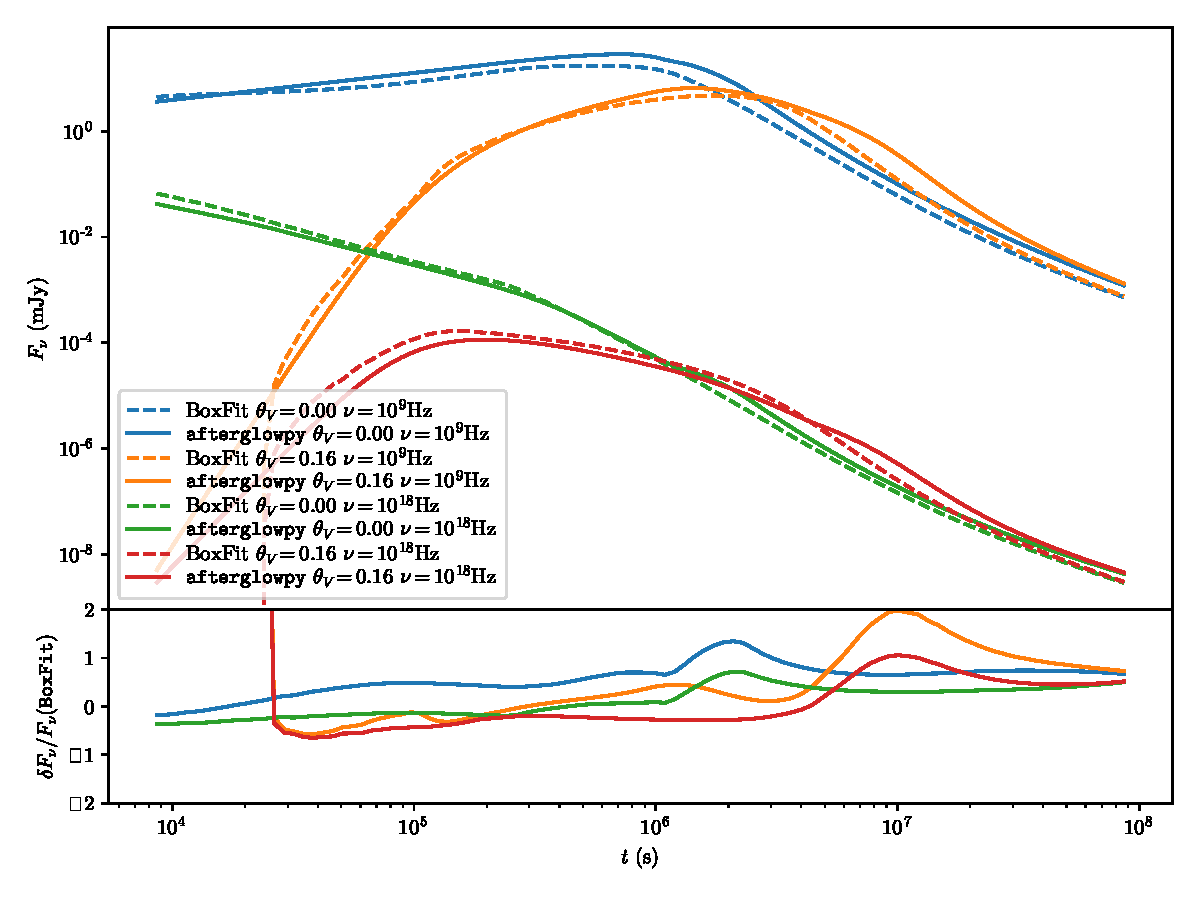
\includegraphics[width=\textwidth]{figs/boxfit_comp.pdf}
	\caption{Top Panel: Comparison between top hat jet light curves from \afterglowpy{} (solid lines) and \boxfit{} (dashed lines). Bottom Panel: Fractional difference between \afterglowpy{} and \boxfit{} light curves.  Four representative light curves are shown: radio on-axis ($\thobs=0$, $\nu=10^9$Hz, blue), radio off-axis ($\thobs=0.16$rad, $\nu=10^9$Hz, orange), x-ray on-axis ($\thobs=0$, $\nu=10^{18}$Hz, green), and x-ray off-axis ($\thobs=0.16$rad, $\nu=10^{18}$Hz, red).  Remaining parameters are shared: $\thC=0.1$rad, $\Eiso=10^{52}$erg, $n_0 = 10^{-3}$cm$^{-3}$, $p=2.2$, $\epse=10^{-1}$, $\epsB=10^{-2}$, $\dL=3.09 \times 10^{26}$cm, $z=0.028$. \label{fig:boxfitComp}}
\end{figure*}

Figure \ref{fig:boxfitComp} shows a comparison between top-hat light curves calculated with \afterglowpy{} and \boxfit{}.   Figure \ref{fig:boxfitComp} shows the light curve of a $\thC=0.1$ rad top-hat jet at radio and x-ray frequencies ($10^9$Hz and $10^{18}$Hz, respectively) with aligned ($\thobs = 0$) and misaligned ($\thobs=0.16$rad) viewing angles.  The light curves begin in the ultra relativistic Blandford-Mckee phase and continue to the Newtonian Sedov phase.

The overall agreement is good: \afterglowpy{} captures the salient features of both aligned and misaligned light curves including the jet break, spectral shape, transition to the Sedov phase, and the early steep rise for misaligned viewing.  
At early times, \boxfit{} lacks the simulation coverage to produce accurate fluxes, leading to a large discrepancy.  Once proper coverage is attained, \boxfit{} and \afterglowpy{} show less than 50\% relative discrepancy until the jet break passes and jet spreading begins.  After the jet break the \afterglowpy{} light curves show a marked excess relative to \boxfit{}, the relative error increasing to approximately 1.0 and 2.0 for the aligned and misaligned radio light curves, respectively.  The x-ray light curves achieve approximately half the error of the radio.  After a short period the \afterglowpy{} light curves begin to decrease, recovering the \boxfit{} slope, and asymptote to similar light curves in the Newtonian regime with a small constant offset from \boxfit{}.

As expected, \afterglowpy{} models the early and late afterglow well, but struggles in an intermediate phase during jet spreading.  In particular it appears that \afterglowpy{} begins its spreading late relative to \boxfit{}.  This phase is precisely where the non-linear hydrodynamics of the blast wave are most important, and hardest to model with simple semi-analytic approximations.  Any work utilizing \afterglowpy{} should be aware of this fact, and be careful when treating data from this regime.

It bears pointing out that some of the hard discrepancy between the codes is due to the test itself: the sharp-edged nature of the top-hat jet exacerbates discrepancies in how these edges are treated.  An angularly structured jet with non-trivial $E(\theta)$ may smooth over the differences in approach between the codes: we may expect \afterglowpy{} to be more accurate for structured jets than top-hats.  \afterglowpy{} is by no means a replacement for full numerical simulations, but is a useful and flexible tool which captures much of the important physics of GRB afterglows at a very small fraction of the cost of a relativistic numerical hydrodynamic simulation.

\afterglowpy{} is available on PyPI and may be installed with {\tt pip}.  The source code is open and available at \url{https://github.com/geoffryan/afterglowpy}.

%%%%%%%%%%%%%%%%%%
%
% Afterglows Section
%
%%%%%%%%%%%%%%%%%%%%

\section{Structured Jet Light Curves}\label{sec:structuredJets}

To fully characterize the light curves of structured jets we use \afterglowpy{} to construct light curves exploring dependence on jet structure model, viewing angle $\thobs$, opening angle $\thC$, and synchrotron regime.  

Using the definition of $\thC$ in Equation \eqref{eq:thCdef} we may write the angular energy profile near the jet axis as:
\begin{equation}
	E(\theta) = E_0 \left (1 - \frac{\theta^2}{2\thC^2} \right) + \OO(\theta^3) \label{eq:EthetaNear}
\end{equation}

The light curves of structured jets show two modes of behaviour, depending on whether the observer is \emph{aligned} ($\thobs < \thC$) or \emph{misaligned} ($\thobs > \thC$).
In the \emph{aligned} case, the light curves follow the standard on-axis top hat behaviour modified slightly for non-zero viewing angle.  There is little to distinguish between different structure $E(\theta)$, and the light curve is well-approximated by a broken power law with characteristic break times \citep{Granot:2002aa}.  The \emph{misaligned} light curve also may present as a broken power law, but with closure relations explicitly dependent on viewing angle and jet angular structure.  

We discuss aligned evolution in detail in Section \ref{subsec:aligned} and misaligned in Section \ref{subsec:misaligned}.  In both cases the transition between phases of evolution depends on the effective solid angle $\Delta \Omega$ of the patch of blast wave dominating the emission.  The size of this patch tends to scale with the Lorentz factor $\gamma$ of the dominant region as:
\begin{equation}
	\Delta \Omega = \gamma^{-\som} \ .
\end{equation}
The parameter $\som$ controls the growth rate of the visible patch, and is typically between 0 and 2. 

\subsection{Aligned Evolution: $\thobs \lesssim \thC$} \label{subsec:aligned}

The aligned light curve of a structured jet is essentially identical to that of a standard top-hat viewed within the jet cone. (CITE Panaitescu \& Kumar).  The relativistic afterglow is comprised of three phases, \emph{pre-jet break}, \emph{transition}, and \emph{post-jet break}.  These are well described in the literature and are briefly reviewed here.

\emph{Pre-jet break} ---  At early times the flux is dominated by the small patch of material whose emission is beamed towards the observer of angular width $\psi = |\theta-\thobs| \sim \gamma^{-1}$.  This patch is within the $\theta < \thC$ region where $E(\theta) \approx E_0$ and the structure plays a sub-dominant role.  The angular size of the visible patch grows with $\som = 2$.  Closure relations and scalings of the standard on-axis top-hat apply. (CITE Granot and Sari)

\emph{Transition} ---  When $\gamma^{-1} \sim \thC-\thobs$ the near edge of the jet comes in to view.  Material outside $\thC$ is less energetic and contributes sub-dominantly to the afterglow emission.  The effective visible patch grows more slowly, $\som \lesssim 2$, and the decay of the afterglow steepens slightly. Closure relations and scalings of the standard on-axis top-hat apply only approximately (CITE vanEerten MacFadyen 2010).  

\emph{Post-jet break} ---  When $\gamma^{-1} \sim \thC+\thobs$ the far edge of the jet comes in to view and growth of the visible patch ceases, $\som = 0$.  If the blast wave remains relativistic and non-spreading, the slope of the light curve is reduced by $-3/4$ relative to the pre-jet break slope.  However, in many circumstances the jet break begins when the blast wave is only trans-relativistic and spreading may have begun.  In these cases an analytic treatment of the light curve is slope is more difficult, but numerical simulations and analytic work estimate an additional reduction of "???" over the simple analytic result.

The transition between pre-jet break and post-jet break begins at $\tbm$ and completes at $\tbp$, given in the single shell approximation (see Appendix \ref{app:derive1}) by:
\begin{align}
	\tbpm &= \left(\frac{9}{16\pi} \frac{E_0}{n_0 \Mp c^5}\right)^{1/3} \left( 2 \sin \left(\frac{\thC\pm\thobs}{2}\right)\right)^{8/3} .\label{eq:tbpm}
\end{align}
\begin{figure}
	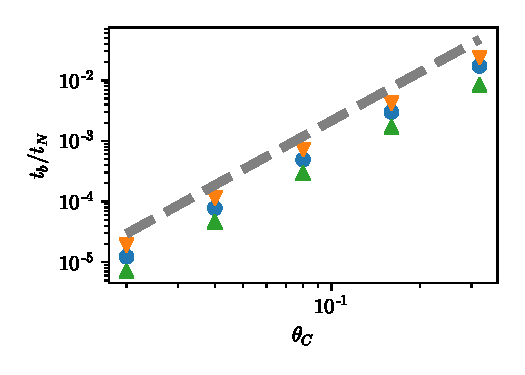
\includegraphics[width=\columnwidth]{figs/breaks_alignedOA_all.pdf}
	\caption{Jet break time for on-axis ($\thobs=0$) observers for top-hat (blue circles), Gaussian (orange squares), and power law (green triangles) jets as a function of $\thC$. The dashed grey line is the analytic approximation $\tbpm = t_N (2\sin \thC/2)^{8/3}$. These particular light curves use $\thW = 5 \thC$, $E_0 = 10^{52}$erg, $n_0=10^{-3}$cm$^{-3}$, $p=2.2$, $\epse = 10^{-1}$, and $\epsB = 10^{-4}$. \label{fig:tbOA}}
\end{figure}

It is important to note that when $\thobs \neq 0$ the transition period is extended, and the most significant transition in the light curve occurs at $\tbp$, the \emph{jet break}.  The jet break occurs, in all jets, when the effective angular size of the visible patch of the jet ceases to increase, that is when $\som = 0$.  

Figure \ref{fig:tbOA} shows the jet break time for on-axis ($\thobs = 0$) viewers as a function of $\thC$ for top-hat, Gaussian, and power law jets calculated with \afterglowpy{}. Break times were extracted by fitting the numerical light curve with a two-component broken power law.

\begin{figure}
	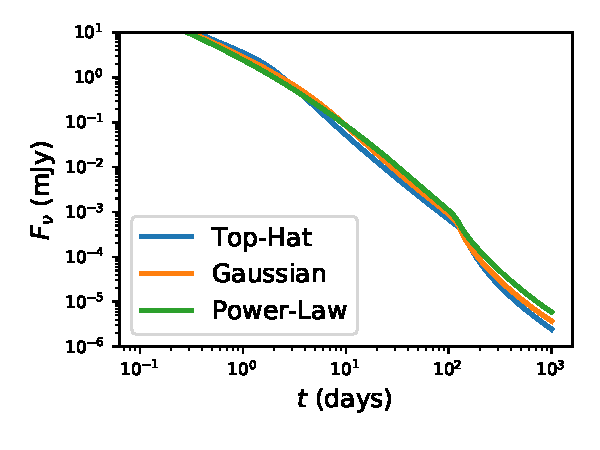
\includegraphics[width=\columnwidth]{figs/lc_on.pdf}
	\caption{Aligned ($\thobs = \thC/2$) afterglow light curves for top-hat (blue), Gaussian (orange), and power law (green) jets. When viewed on-axis, jets containing angular structure are very difficult to distinguish from top-hats.  The transition phase marking the onset of the jet break begins at $\tbm\sim3$ days with a shallow break and ends sharply at $\tbp \sim 100$ days.  These particular light curves use $\thC = 0.1$ rad, $\thW = 0.4$ rad, $E_0 = 10^{52}$erg, $n_0=10^{-2}$cm$^{-3}$, $p=2.2$, $\epse = 10^{-1}$, $\epsB = 10^{-3}$, and $d_L=40$Mpc. \label{fig:onaxis}}
\end{figure}

\begin{figure*}
	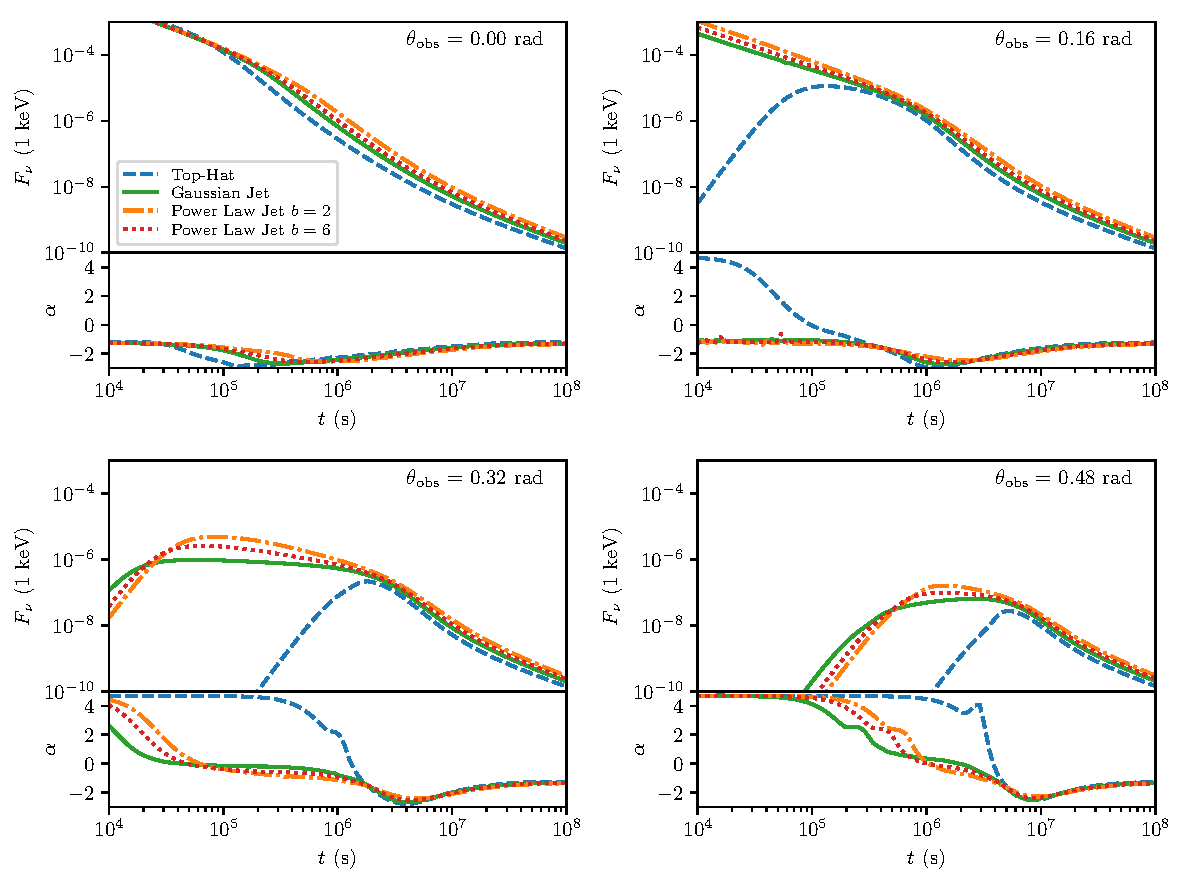
\includegraphics[width=\textwidth]{figs/lc_thV_model_multi.pdf}
	\caption{X-ray afterglow light curves from structured jets at different viewing angles $\thobs$, calculated with \afterglowpy{}.  Each panel shows the 1 keV flux density $F_\nu$ and the corresponding temporal slope $\alpha = d\log F_\nu / d\log \tobs$.  Included models are the top-hat jet (dashed blue), Gaussian jet (solid green), $b=2$ power law (dot-dashed orange), and $b=6$ power law at $\thobs=0$ (upper left), $\thobs=2\thC=0.16$ rad (upper right), $\thobs=4\thC=0.32$ rad (lower left), and $\thobs=6\thC=0.48$ rad (lower right). These particular light curves all use $\thC = 0.08$ rad, $\thW = 0.24$ rad, $E_0 = 10^{53}$erg, $n_0=1$ cm$^{-3}$, $p=2.2$, $\epse = 10^{-1}$, $\epsB = 10^{-2}$, $d_L=10^{28}$cm and $z=0.5454$. \label{fig:thVmodel}}
\end{figure*}

Figure \ref{fig:onaxis} shows representative top-hat, Gaussian, and power law jet light curves in the aligned regime.  The light curves nearly overlap, demonstrating the similar evolution of all structured jet afterglows when viewed within the jet core.  Although we expect all afterglow blast waves to contain angular structure, the simple top-hat jet model is sufficient for aligned viewing.

The relativistic stages of evolution are followed by a Newtonian phase ($t > 200$ days in Figure \ref{fig:onaxis}) when the decelerating blast wave becomes non-relativistic, spreads sonically, and approaches a Sedov-Taylor solution.  We do not address the Newtonian phase of evolution in this work.

\subsection{Misaligned Evolution: $\thobs \gtrsim \thC$} \label{subsec:misaligned}

When viewed at angles larger than $\thC$ the gradient $E'(\theta)$ over the visible patch becomes non-negligible.  To observers this energy gradient presents itself as a slowly rising or decaying afterglow light curve. The relativistic afterglow is comprised of two or three phases depending on whether the observer lies within the truncation angle, \emph{far off-axis}, \emph{structured}, and \emph{post-jet break}.

\emph{Far off-axis} --- If the viewer lies outside the truncation angle, $\thobs > \thW$, then at early times the entire blast wave surface is off-axis and all emission is beaming suppressed.  This greatly reduces the early flux and leads to a dim but steeply rising light curve as the blast wave decelerates.  Emission is dominated by material on the edge nearest the observer and the angular size of the visible patch is constant in time.  This phase ends at $\tW$ when $\gamma^{-1} \sim \thobs-\thW$.  If $\thobs < \thW$ this phase is entirely absent.  Table \ref{tab:slopes} gives the temporal power law slope of the light curve in this phase.  These slopes are derived in Appendix \ref{app:derive1}.

\emph{Structured} --- The structured phase is the direct result of the energy gradient along the observer's line of site.  The usual (pre-jet break) decay is compensated for by regions of higher energy continuously coming into view as the jet decelerates.  These new contributions to the emission slow the decay and can even cause the observed flux to increase with time.

 This phase begins at observer time $\tW$, once the blast wave is decelerating and the observer is within the beaming cone of any part of the emitting surface.  It ends at observer time $\tb$, when the jet core has become fully visible.  These times are:
\begin{align}
	\tW &= \left(\frac{9}{16\pi} \frac{E(\thW)}{n_0 \Mp c^5}\right)^{1/3} \left( 2 \sin \left(\frac{\thobs-\thW}{2}\right)\right)^{8/3} \ ,\label{eq:tw} \\
	\tb &= \left(\frac{9}{16\pi} \frac{E_0}{n_0 \Mp c^5}\right)^{1/3} \left( 2 \sin \left(\frac{\thobs}{2}\right)\right)^{8/3} \ .\label{eq:tb}
\end{align}

\begin{figure}
	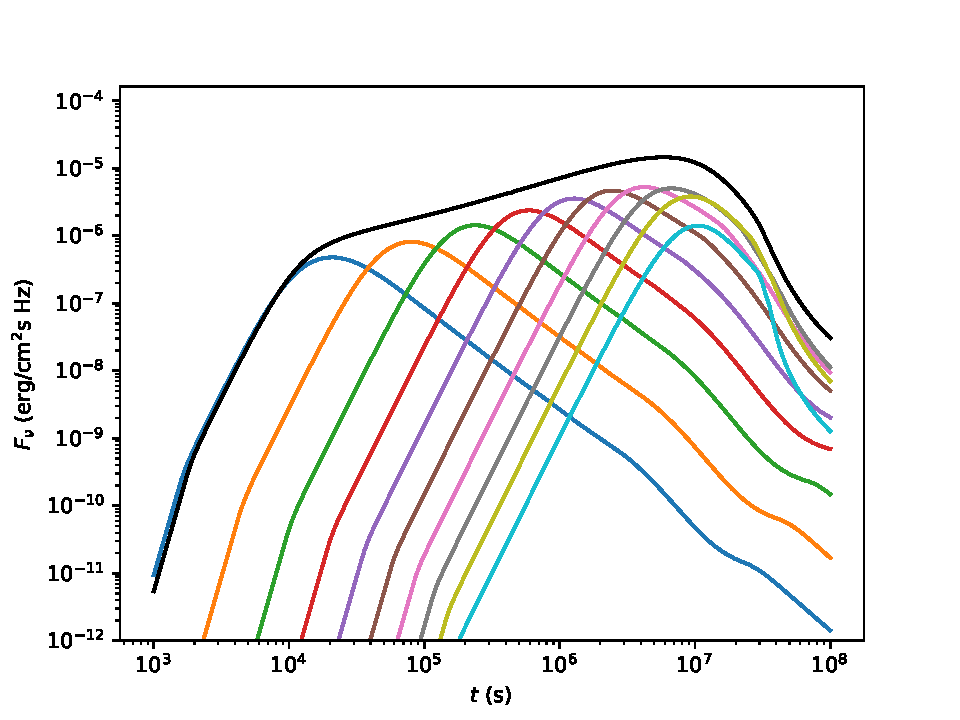
\includegraphics[width=\columnwidth]{figs/jetDecomp.pdf}
	\caption{A Gaussian structured jet, decomposed into emission from different latitudes $\theta$.  The off-axis, structured, and post-jet break phases are all clearly visible.  The structured phase is the result of the brightest point of the blast-wave tracking from the wings $(\theta =\thW$) to the jet core ($\theta=\thC$). \label{fig:decomp}}
\end{figure}
Figure \ref{fig:decomp} shows the light curve of a Gaussian structured jet along with the emissions from different latitudes.  The part of the blast wave dominating the emission tracks from the high latitude wings $\theta \approx \thW$ to the core $\theta \approx 0$. The angular size of the visible patch grows approximately as $\gamma^{-1.0}$. (NEED PLOT?)

During the structured phase, the afterglow has a temporal spectral slope which depends on the parameter $g(\theta^*)$, where $\theta^*$ is the latitude of material dominating the emission:
\begin{equation}
	g(\theta^*) \equiv -2 \tan\left(\frac{\thobs - \theta^*}{2}\right)\frac{d \log E}{d \theta}\ . \label{eq:gdef}
\end{equation}

The temporal and spectral slopes for various regimes are given in Table \ref{tab:slopes}.  The derivation of the closure relations, $\tW$, and $\tb$ are given in Appendix \ref{app:derive1}.

\begin{deluxetable*}{CCCCCCC}
	\tablecaption{Structured jet temporal and spectral slopes: $F_\nu \propto \tobs^{-\alpha} \nu^{-\beta}$. See Equations \eqref{eq:gdef} and \eqref{eq:geff} for the definition and effective values of $g$. \label{tab:slopes}}
	\tablehead{\colhead{Regime}& \colhead{Label} & \colhead{$\alpha_{\mathrm{off-axis}}$}& \colhead{$\alpha_{\mathrm{struct}}$}& \colhead{$\alpha_{\mathrm{struct,max}}$}& \colhead{$\alpha_{\mathrm{post, analytic}}$} & \colhead{$\beta$}}
	\startdata
	\nu<\nu_m<\nu_c     & D & 7 			& \frac{1 + 3g}{8+g} 		& 3		& -1/4		& 1/3 \\
	\nu_m<\nu<\nu_c     & G & 15/2 - 3p/2 	& \frac{3 - 6p +3g}{8+g} 	& 3		& -3p/4		& (1-p)/2 \\
	\nu < \nu_c < \nu_m & E & 17/3 		& \frac{-5/3 + 11g/3}{8+g} 	& 11/3	& -7/12		& 1/3 \\
	\nu_c < \nu < \nu_m & F & 13/2 		& \frac{-5 + 2g}{8+g} 		& 2		& -1			& -1/2 \\
	\nu_c < \nu_m < \nu & H & 8 - 3p/2 		& \frac{1-6p  +2g}{8+g} 	& 2		& -(3p+1)/4	& -p/2 \\ 
	\enddata
\end{deluxetable*}


%\begin{deluxetable*}{CCCCCC}
%	\tablecaption{Structured jet temporal and spectral slopes: $F_\nu \propto \tobs^{-\alpha} \nu^{-\beta}$. See Equations \eqref{eq:gdef} and \eqref{eq:geff} for the definition and effective values of $g$.  For a refreshed-shock model replace $g$ with $k$, defined in Equation \eqref{eq:Eu}. \label{tab:generalSlopes}}
%	\tablehead{\colhead{Regime}& \colhead{Label} & \colhead{$\alpha_{\mathrm{off-axis}}$}& \colhead{$\alpha_{\mathrm{struct}}$}& \colhead{$\alpha_{\mathrm{struct,max}}$} & \colhead{$\beta$}}
%	\startdata
%	\nu<\nu_m<\nu_c     & D & -7 			& -\frac{-2+3s_3 + 3g}{8+g} 		& -3		& -1/3 \\
%	\nu_m<\nu<\nu_c     & G & -15/2 + 3p/2 	& -\frac{- 6p + 3s_3 + 3g}{8+g} 		& -3		& (p-1)/2 \\
%	\nu < \nu_c < \nu_m & E & -17/3 		& -\frac{-14/3 + 3s_3 + 11g/3}{8+g} 	& -11/3	& -1/3 \\
%	\nu_c < \nu < \nu_m & F & -13/2 		& -\frac{-8+3s_3 + 2g}{8+g} 		& -2		& 1/2 \\
%	\nu_c < \nu_m < \nu & H & -8 + 3p/2 		& -\frac{-6p - 2 + 3s_3 + 2g}{8+g} 	& -2		& p/2 \\ 
%	\enddata
%\end{deluxetable*}

The $g$ parameter evolves with time as $\theta^*$ sweeps from the jet edge to the core.  This produces deviations in the light curve from a pure power law.  However, we find ultimately these deviations are not too large and the average slope is well approximated by $\geff  = g(\thobs/2)$.  For the power law and Gaussian jet models this gives:
\begin{align}
	\theff &= \frac{\thobs}{2}&& \text{Gaussian}\ , \\
	\theff &= \frac{\thobs}{\sqrt{1.8+2.1b^{-1.25} + (0.49-0.86b^{-1.25})\thobs/\thC}}&& \text{power law}\ . \label{eq:theff}
\end{align}
\begin{align}
	\geff &= \frac{\thobs^2}{4\thC^2} && \text{Gaussian}\ , \\
	\geff &= \frac{b \thobs^2}{4 \thC^2+\thobs^2} && \text{power law}\ . \label{eq:geff}
\end{align}
These values may be used in Table \ref{tab:slopes} for an approximate power law model of a structured jet with an appropriate viewing angle dependent temporal evolution.  These analytic results are in agreement with previous work on structured jets (CITE ROSSI) and the trans-relativistic numerical model described in Section \ref{sec:numerical}.

In the structured phase, the temporal slope depends directly on the ratio $\thobs/\thC$.  Therefore any measurement of the effective power law slope of an afterglow light curve in the structured phase can be used to measure this parameter.

\emph{Post-jet break} --- Once the entire jet is visible (ie. the observer is within the beaming cone of the entire jet) the visible patch no longer grows and emission is dominated by the decelerating core.  This phase follows exactly the post-jet break scalings of the aligned case, except with a much delayed break time $\tb$.

\begin{figure}
	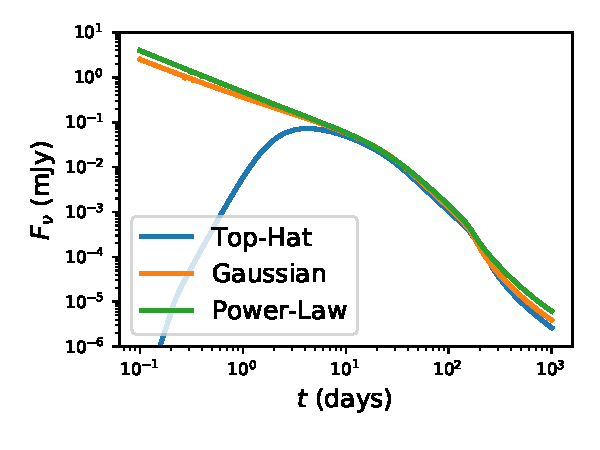
\includegraphics[width=\columnwidth]{figs/lc_off1.pdf}
	\caption{As Figure \ref{fig:onaxis} but $\thobs = 2\thC$.  The top-hat jet (with opening angle $\thC$) begins in the off-axis phase.  The Gaussian and power law jets begin in the structured phase as $\thobs < \thW$.  All three models enter similar post-jet break phases. \label{fig:offaxis1}}
\end{figure}
\begin{figure}
	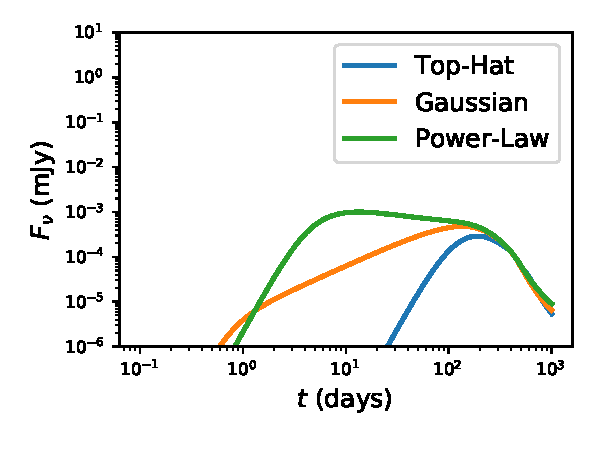
\includegraphics[width=\columnwidth]{figs/lc_off2.pdf}
	\caption{As Figure \ref{fig:onaxis} but $\thobs = 6\thC$. All three models exhibit off-axis, structured, and post-jet break phases of evolution.  At larger opening angles the difference between structured models is more evident.  \label{fig:offaxis2}}
\end{figure}

Figures \ref{fig:offaxis1} and \ref{fig:offaxis2} display afterglows from the fiducial models in the misaligned regime at $\thobs = 2\thC$ and $\thobs=6\thC$ respectively.  At the moderate $2\thC$ viewing angle both structured models exhibit similar decaying light curves with slopes somewhat shallower than the aligned case. In this case $\thobs < \thW$ so neither model exhibits an off-axis phase.  The similar temporal evolution is easy to understand as at this angle both models have $\geff = 1$ and hence approximately equal power law slopes in the structured phase.  At late times as more of the jet comes in to view the difference between all three models becomes negligible. 

At the larger $6\thC$ viewing angle all three models exhibit off-axis, structured, and post-jet break phases of the afterglow.  The different $\tW$ between the Gaussian and power law models is due to the different $E(\thW)$ of the two models. In the structured phase the Gaussian shows a rising light curve with slope $~1$ due to the large $\geff = 9$.  The power law meanwhile has a smaller $\geff$ of $9/5$, giving rise to a very shallow decay. As at the other viewing angles, once the entire jet is visible at $\tb$ all models follow similar post-jet break evolutions.

%
% Comment: Add dashed line at 0 to slopes plot.
%

\begin{figure}
	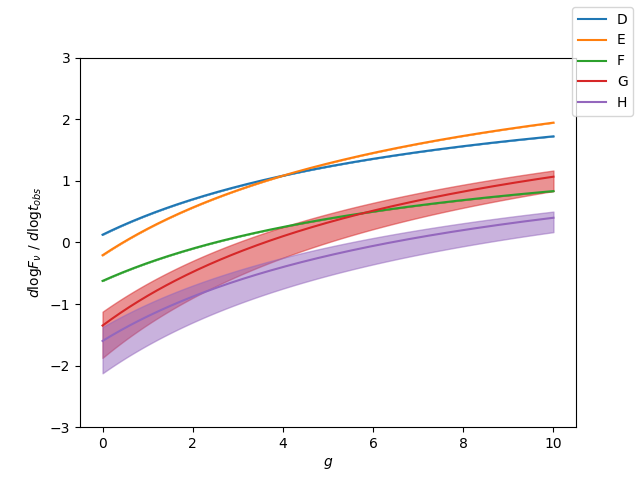
\includegraphics[width=\columnwidth]{figs/slopesJet.png}
	\caption{Temporal slopes for the off-axis structured jet as a function of the structure parameter $g$ for the synchrotron spectral regimes D (blue, narrow), E (orange, narrow),  F (green, narrow), G (red, wide), and H (purple, wide).  The width of the G and H bands shows the dependency on $p$, the upper curves for $p=2$ and the lower for $p=3$.  The temporal power law slope of a structured jet afterglow increases with $g$ in all spectral regimes. \label{fig:slopesG}}
\end{figure}

Figure \ref{fig:slopesG} shows the structured phase power law temporal slope as a function of $g$ for spectral regimes $D$--$H$. In the $G$ and $H$ regimes the spectral slope is a function of $p$, this dependence carries over into the temporal slope as well. The temporal slope is an increasing function of $g$ in all regimes.  At sufficiently large $g$ all regimes exhibit rising light curves, the specific $g$ at which the light curve begins to rise is regime dependent.

\subsection{Refreshed Shocks --- Fast Tails and Spherical Cocoons}\label{subsec:refreshedShocks}

An alternative mechanism to produce slow decays or rises in afterglow light curves is the \emph{refreshed shock}, where velocity stratification of the ejecta causes a prolonged period of energy injection in the afterglow.  This material may be a tail of fast outflowing ejecta or ejecta material accelerated through interaction with a possibly choked jet (e.g. a cocoon). (CITE Mooley, Hotokezaka, Nakar\&Piran, etc).  In either case, slow material initially coasting behind the shock is gradually incorporated into the blast wave as it decelerates, ``refreshing'' the shock.  This mechanism was first proposed as an energy injection scenario (CITE), and was proposed as the mechanism behind the \gwbns{} afterglow in the choked-jet scenario. (CITE Mooley, Hotokezaka, etc).

In the simplest case the visible part of the blast wave is assumed to be quasi-spherical.  The velocity distribution of material behind the blast wave is specified by $E_{>}(u)$, the energy of all material in the ejecta with four-velocity greater than $u$.  This is typically taken to be a power law in $u$ within the finite domain $[\umin, \umax]$:
\begin{equation}
	E_>(u) = E_r u^{-k}\ , \label{eq:Eu}
\end{equation}
where $u \in (\umin, \umax)$ is the dimensionless four-velocity, $k>0$ is the power law index, and $E_r$ is a normalization factor.  The mass ejected with velocity $\umax$ is $\Mej$.

%
% Comment: define tdec, tmin IN THE TEXT.   Add (brief) discussion of light curve phases.
%

A blast wave will have an initial coasting period before sweeping up enough mass in the ambient medium to begin deceleration and be subject to refreshed shocks.  The transition between coasting and decelerating occurs in the bursters frame at $\tdec$. The shock refreshment ends when the blast wave decelerates past $\umin$, in the observers frame at $\tumin$.  In the single shell model with trans-relativistic equation of state used here, these times are:
\begin{align}
	\tdec &= \left(\frac{9}{4\pi} \frac{\Mej}{n_0 \Mp c^3} \frac{\gmax^2}{\bmax^3(\gmax+1)(4\umax^2+3)} \right)^{1/3}  \ ,\label{eq:tdec} \\
	\tumin &= \left(\frac{9}{16\pi} \frac{E_r}{n_0 \Mp c^5}\right)^{1/3} \umin^{-8/3} \ .\label{eq:tumin}
\end{align}
Equation \eqref{eq:tumin} assumes $E_r \gg \Mej c^2$.   The temporal and spectral slopes in this mechanism depend on the energy distribution index $k$ and are given in Table \ref{tab:refreshSlopes}.  Figure \ref{fig:slopesK} shows the temporal slopes in each spectral regime as a function of $k$.  As in Figure \ref{fig:slopesG} the width of the $G$ and $H$ regimes reflects varying the value of $p$ between two and three.  For a derivation see Appendix \ref{app:derive3}.  


%
% Comment: Add dashed line at 0 to slopes plot.
%


\begin{figure}
	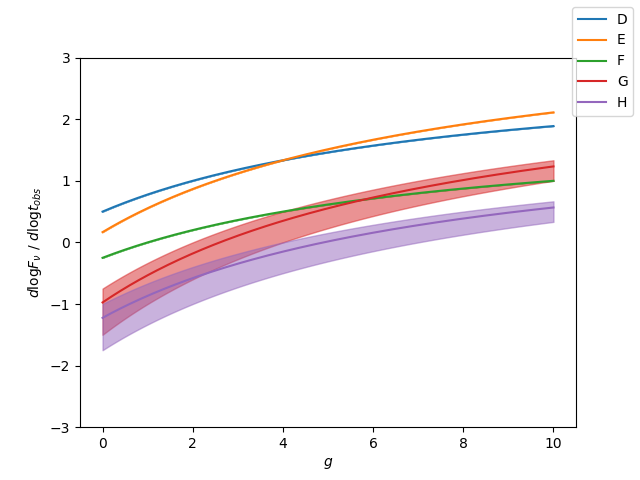
\includegraphics[width=\columnwidth]{figs/slopesCocoon.png}
	\caption{The temporal power law slope of the spherical refreshed-shock afterglow light curve as a function of $k$.  Otherwise as Figure \ref{fig:slopesG}.  The temporal power law slope of a structured jet afterglow increases with $k$ in all spectral regimes. \label{fig:slopesK}}
\end{figure}

\begin{deluxetable*}{CCCCCCC}
	\tablecaption{Refreshed shock temporal and spectral slopes: $F_\nu \propto \tobs^{-\alpha} \nu^{-\beta}$. See Equation \eqref{eq:Eu} for the definition of $k$.  \label{tab:refreshSlopes}}
	\tablehead{\colhead{Regime}& \colhead{Label} & \colhead{$\alpha_{\mathrm{coast}}$}& \colhead{$\alpha_{\mathrm{refresh}}$}& \colhead{$\alpha_{\mathrm{refresh,max}}$}& \colhead{$\alpha_{\mathrm{post}}$}  & \colhead{$\beta$}}
	\startdata
	\nu<\nu_m<\nu_c     & D & 3 	& -\frac{4 + 3k}{8+k} 		& -3		& -1/2	& -1/3 \\
	\nu_m<\nu<\nu_c     & G & 3 	& \frac{-6 + 6p - 3k}{8+k} 	& -3		& 3(p-1)/4	& (p-1)/2 \\
	\nu < \nu_c < \nu_m & E & 3 	& -\frac{4/3 + 11k/3}{8+k} 	& -11/3	& -1/6	& -1/3 \\
	\nu_c < \nu < \nu_m & F & 3 	& \frac{2 - 2k}{8+k} 		& -2		& 1/4		& 1/2 \\
	\nu_c < \nu_m < \nu & H & 3 	& \frac{- 4 +6p - 2k}{8+k}	& -2		& (3p-2)/4	& p/2 \\ 
	\enddata
\end{deluxetable*}


\subsection{Relation to Energy Injection Models}

The light curves of both the misaligned angularly structured jet and refreshed shock models can be understood in terms of general energy injection mechanisms, parameterized as an additional power $L$ delivered to the blast wave.  This power is typically taken to decay in time as a power law, $L \propto t^{-q}$, with $q \in [0,1]$.

The mapping between energy injection and refreshed shocks was done by \cite{Zhang:2006aa}.  That work specifies the index $s$ of the mass distribution $M_{>u} \propto u^{-s}$, which is related simply to the index $k$ by $k = s-1$. Under this mapping the closure relations in Table \ref{tab:slopes} are equivalent to those in \cite{Zhang:2006aa} and the model can be seen as equivalent to an energy injection model with $q = (8-2k) / (8+k)$.

Misaligned structured jets do not map as neatly onto energy injection models as the scaling of the visible patch, $\som = 1.0$, is different than in standard afterglows, $\som = 2$. Once this change is accounted for, the $g$ parameter plays the same role as $k$, as can be seen by a simple comparison between $\alpha_{\text{struct}}$ in Table \ref{tab:slopes} and $\alpha_{\text{refresh}}$ in Table \ref{tab:refreshSlopes}.  That is, a structured jet light curve is equivalent to a standard energy injection model with:
\begin{align}
	q &= (8-2g) / (8+g)  \label{eq:struct2ei} \\
	\som &= 1
\end{align}

Generic closure relations leaving the dependence on $\som$ explicit are presented in Table \ref{tab:generalSlopes}. 


%
% Comment: replace s_3 with s_Omega, s_{1,2} with s_gamma, s_t.
%
% "It is insightful..."
%


%
% Comment: Emphasize this is in "misaligned" case for structured case, but also applies to refreshed shock.  Just use "alpha".
%

%
% Comment: THE JET BREAK *IS* WHEN THE VISIBLE PATCH STOPS GROWING
%

\begin{deluxetable*}{CCCCCC}
	\tablecaption{Generic closure relations for the afterglow of a relativistic blast wave in a homogeneous medium: $F_\nu \propto \tobs^{\alpha} \nu^{\beta}$.  See Equations \eqref{eq:gdef} and \eqref{eq:geff} for the definition and effective values of $g$ for misaligned structured jets.  Jets aligned with the viewer or without angular structure have $g=0$.  The visible patch of the jet has a solid angle which scales as $\gamma^{-\som}$.  A uniform relativistic blast wave pre-jet break has $\som=2$, a relativistic blast wave with angular structure pre-jet break has $\som \approx 1$, and a relativistic blast wave post jet-break has $\som = 0$.  For a refreshed-shock model replace $g$ with $k$, defined in Equation \eqref{eq:Eu}. \label{tab:generalSlopes}}
	\tablehead{\colhead{Regime}& \colhead{Label} & \colhead{$\alpha$} & \colhead{$\beta$}}
	\startdata
	\nu<\nu_m<\nu_c     & D & \frac{-2 + 3\som + 3g}{8+g} 		& 1/3 \\
	\nu_m<\nu<\nu_c     & G & \frac{-6p + 3\som + 3g}{8+g} 	& (1-p)/2 \\
	\nu < \nu_c < \nu_m & E & \frac{-14/3 + 3\som + 11g/3}{8+g} 	& 1/3 \\
	\nu_c < \nu < \nu_m & F & \frac{-8 + 3\som + 2g}{8+g} 		& -1/2 \\
	\nu_c < \nu_m < \nu & H & \frac{-6p - 2 + 3\som + 2g}{8+g} 	& -p/2 
	\enddata
\end{deluxetable*}

\section{Application: \gwbns{}}\label{sec:gw170817}

We use the electromagnetic afterglow of \gwbns{} as an example application of both the analytic and numerical structured jet afterglow models.  

Figure \ref{fig:170817Alc} shows the observations in radio, optical, and x-ray bands of the \gwbns{} afterglow.  No afterglow emission was detected until an x-ray detection by the Chandra observatory nine days after the GW trigger \cite{Troja:2017aa}.  Further radio, optical, and x-ray observations showed a steady rising light curve with constant power law slope until a peak near day 160.  At this point the light curve turned over and began a steep decay that continues to the present \citep{van-Eerten:2018aa}.

Interpreting the afterglow as arising from a structured jet allows one to quickly draw the following conclusions:
\begin{enumerate}
	\item The spectral slope $\beta = 0.585$ (CITE, +uncertainties) throughout the entire evolution, identifying the relevant spectral regime as G: $\nu_m < \nuobs < \nu_c$, and $p = 2.17$.
	\item The initial rising ($\alpha > 0$) light curve with declining spectrum ($\beta < 0$) identify this as a \emph{misaligned} evolution ($\thobs > \thC$).  Aligned jets may only have a rising light curve when viewed at frequencies below the peak frequency, that is when $\beta < 0$.
	\item The rising light curve maintains $\alpha  = 0.90 \pm 0.06$ (CITE YITL).  Using the closure relations from Table \ref{tab:slopes} we can identify this as the \emph{structured} phase and determine $\geff = 7.5 \pm 0.4$.  If the light curve underwent an \emph{off-axis} phase, it concluded before the afterglow was detected: $\tW < 9$d.  The peak can be identified as the jet-break: $\tb = 164 \pm 12$ d.
	\item In the context of a Gaussian jet, the measurement of $\geff$ leads immediately to $\thobs / \thC = 5.5 \pm 0.2$.
	\item Using the Fong 2015 (CITE Fong 2015) fiducial values of $E_0 \sim 2\times 10^{51}$erg and $n_0 \sim 10^{-2}$cm$^{-3}$ we can use the jet break $\tb$ measurement to determine $\thobs \approx 0.5 \pm 0.2$ rad ($29^\circ \pm 12^\circ$), assuming 1 dex uncertainties on $E_0$ and $n_0$.    This is in agreement with the LIGO measurement $\thobs \approx 28^\circ \pm 15^\circ$ (assuming the SHoES $H_0$).
	\item The combined measurements of $\thobs$ and $\thobs/\thC$ then imply $\thC \approx 0.09 \pm 0.04$ rad ($5^\circ  \pm 2^\circ$).
\end{enumerate}

For a more detailed analysis we performed Bayesian parameter estimation utilizing \afterglowpy{} and the \emcee{} Markov chain Monte Carlo sampler \citep{Foreman-Mackey:2013aa}.  We used the light curve data reported in \citet{van-Eerten:2018aa} with additional \hubble{} observations reported in \citet{Lamb:2019aa}. Reported measurement uncertainties were assumed to be independent and Gaussian, upper limits were treated as observations of zero flux with a 1-sigma Gaussian uncertainty. 

We fit both the Gaussian and power law structured jet models, fixing $\xi_N = 1$ and $\dL = 1.23 \times 10^{26}$cm.  The fit parameters, their priors, and their marginalized posteriors are given in Table \ref{tab:MCMC}. Both models were run with 300 walkers for 64 000 iterations, discarding the first 16 000 iterations as a burn-in.  The viewing angle prior is the posterior found in analysis of the \gwbns{} gravitational wave signal assuming the value of $H_0$ reported by the \planck{} collaboration \citep{Abbott:2017aa, Planck-Collaboration:2016aa, Troja:2018aa}.  

\begin{deluxetable*}{CCCCCC}
	\tablecaption{Parameter estimation priors and marginalized posteriors for the \gwbns{} afterglow using the \afterglowpy{} Gaussian and power law jet models, including viewing angle constraints from LIGO assuming the \planck{} value of $H_0$.  Given posterior values for each model are the median, 16\%, and 84\% quantiles.  Parameters in the lower section are derived from the posterior distributions of the fit parameters in the upper sections. \label{tab:MCMC}}
	\tablehead{\colhead{Parameter}& \colhead{Unit} & \colhead{Prior Form} & \colhead{Bounds} & \colhead{Gaussian Jet Posterior} & \colhead{Power Law Jet Posterior}}
	\startdata
		\thobs	& \text{rad	} & \sin \thobs \times p_\mathrm{LIGO}(\cos \thobs)	& [0, 0.8] 	& 0.48^{+0.08}_{-0.09} & 0.36^{+0.14}_{-0.11} \\
		\log_{10} E_0	& \text{erg	}	& \text{uniform}	& [45, 57] 			& 52.92^{+0.62}_{-0.49} & 53.01^{+0.99}_{-0.70}\\
		\thC			& \text{rad	}	& \text{uniform}	& [0.01, $\pi/2$]		& 0.07^{+0.01}_{-0.01} & 0.10^{+0.06}_{-0.03}\\
		\thW			& \text{rad}	& \text{uniform}	& [0.01, 12$\thC$]	& 0.77^{+0.43}_{-0.38} & 0.18^{+0.07}_{-0.05}\\
		b			& - 			& \text{uniform}	& [0, 10] 			& - & 7.15^{+2.02}_{-1.12}\\
		\log_{10}n_0	& \text{cm}^{-3} & \text{uniform}	& [-10, 10] 		& -1.94^{+0.62}_{-0.65} & -2.66^{+1.03}_{-1.11}\\
		p			& - 			& \text{uniform}	& [2, 5] 			& 2.17^{+0.01}_{-0.01} & 2.17^{+0.01}_{-0.01}\\
		\log_{10}\epse& - 			& \text{uniform}	& [-5, 0] 			& -1.24^{+0.48}_{-0.69} &-1.30^{+0.66}_{-1.07} \\
		\log_{10}\epsB	& - 			& \text{uniform}	& [-5, 0] 			& -4.32^{+0.72}_{-0.49} & -3.84^{+1.01}_{-0.80}\\
		\hline
		\log_{10}\Etot	& \text{erg}	&	-		&	-			& 50.61^{+0.58}_{-0.44} &50.85^{+0.93}_{-0.63} \\
		\thobs/\thC	& -			&	-		&	-			& 6.76^{+0.21}_{-0.21} & 3.78^{+0.58}_{-0.84}\\
	\enddata
\end{deluxetable*}

\begin{figure*}
	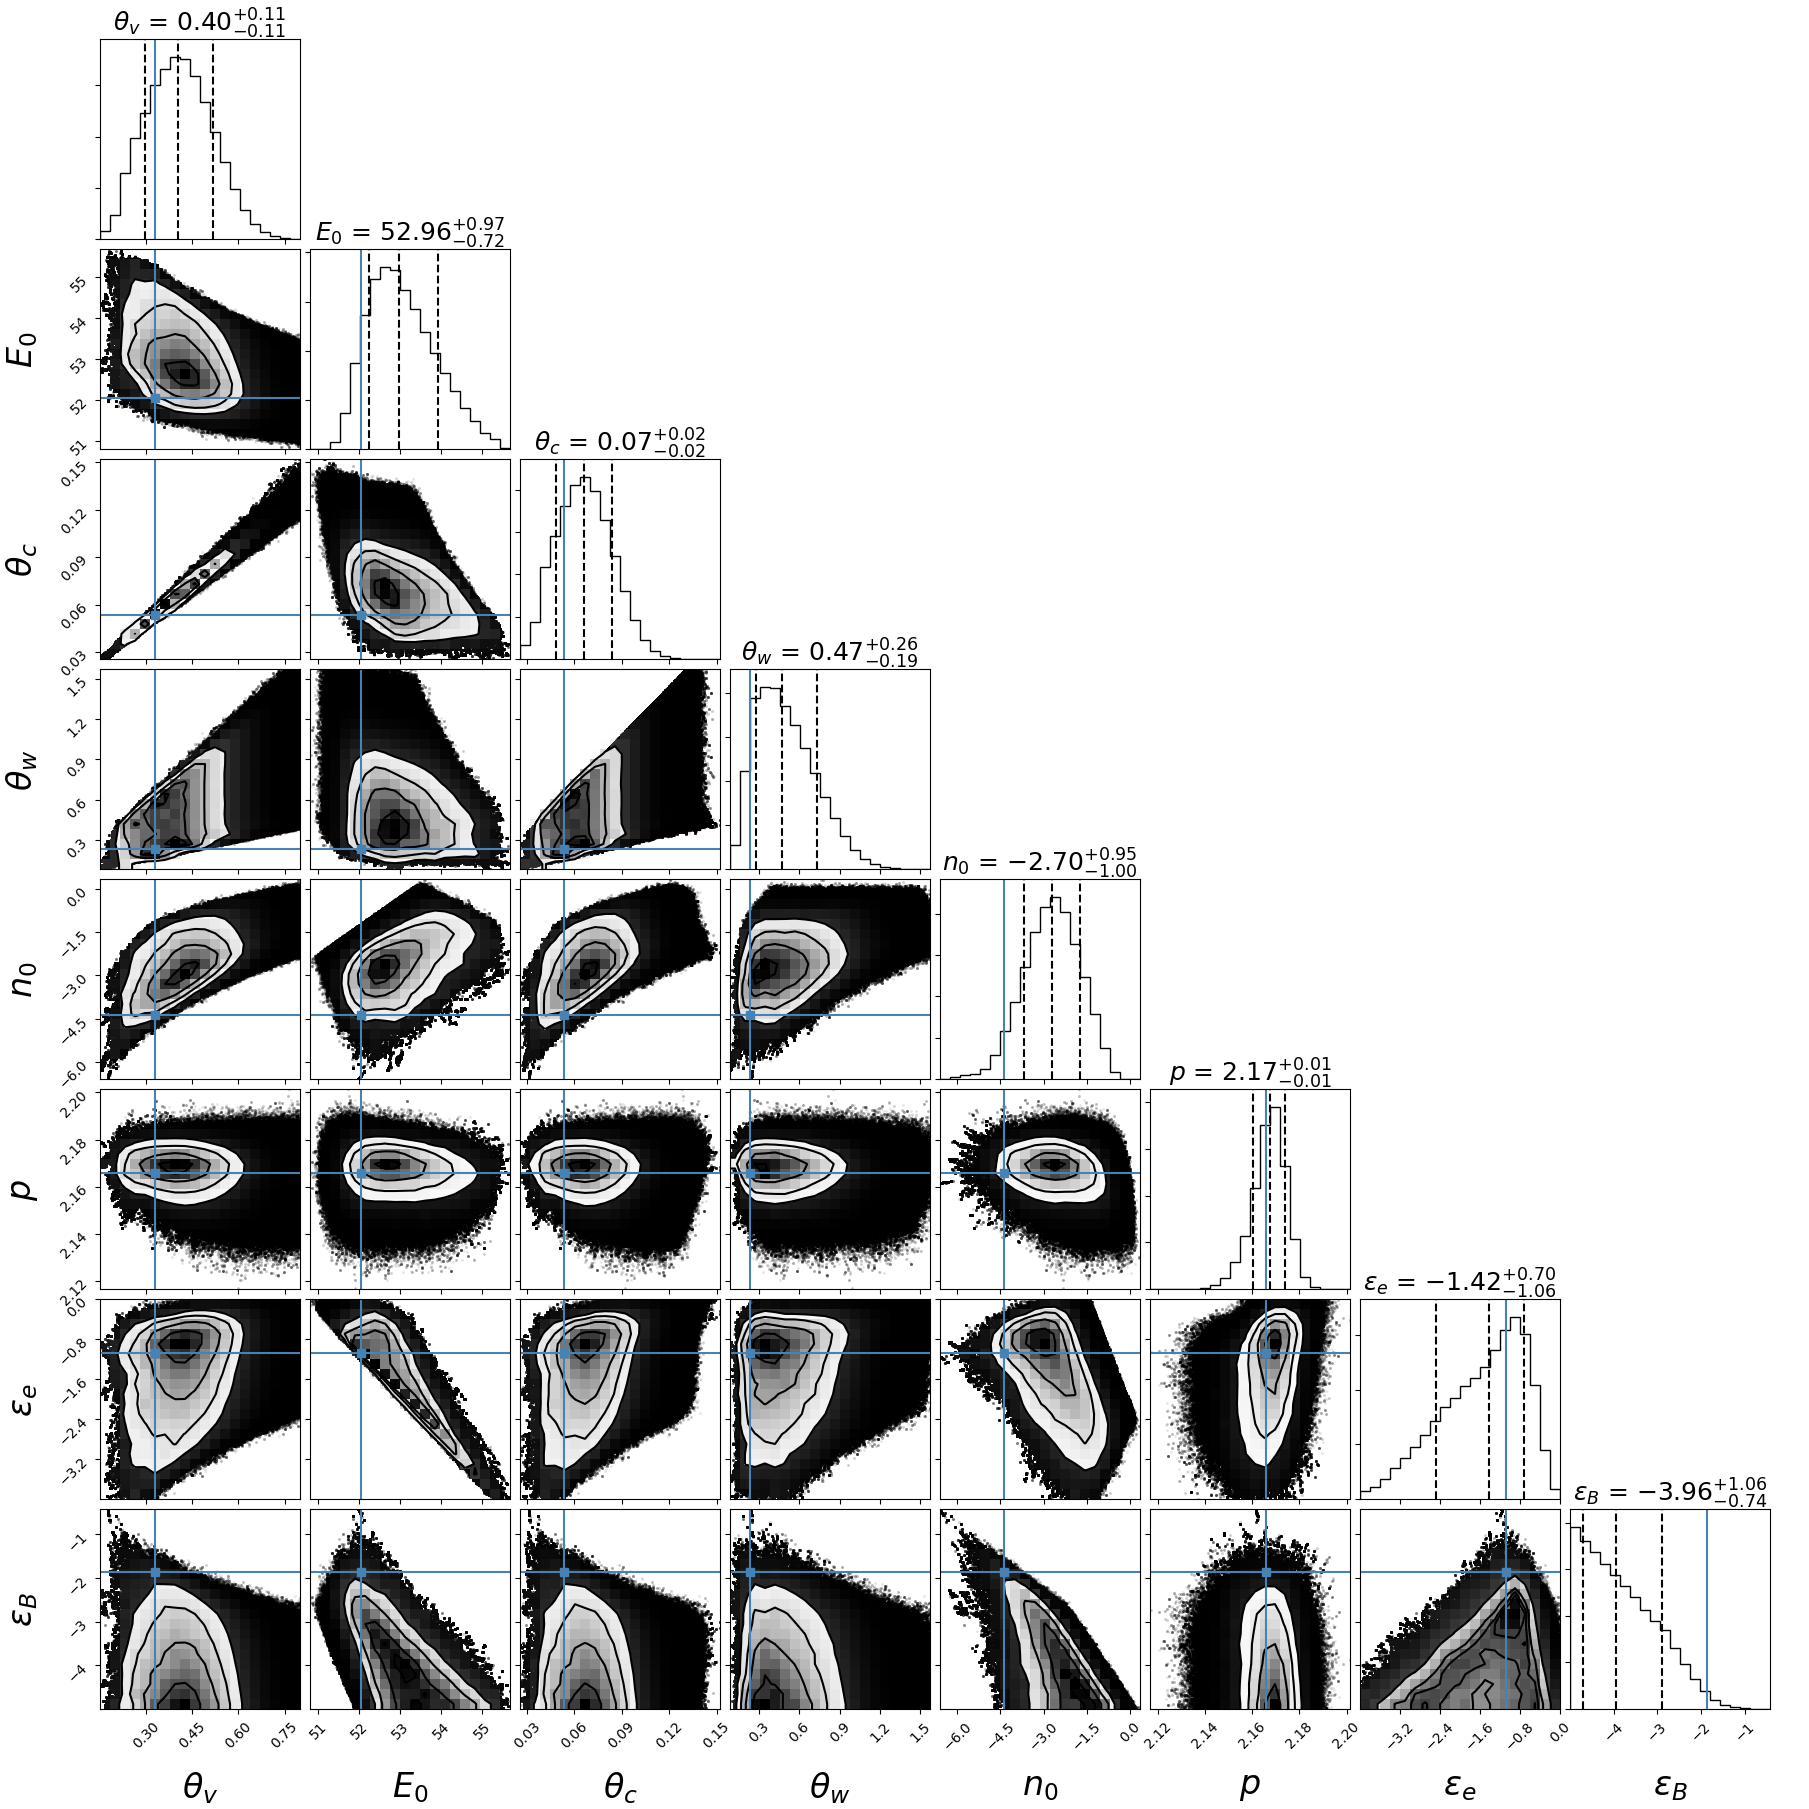
\includegraphics[width=\textwidth]{figs/cornerGaussian.png}
	\caption{Views of the posterior parameter distribution for a Gaussian jet fit to the \gwbns{} afterglow.  The diagonal contains one-dimensional marginalized posteriors for each fit parameter, while the off-diagonal plots contain two-dimensional maps of the posterior marginalized over all but the two corresponding parameters. \label{fig:cornerGaussian}}
\end{figure*}

\begin{figure*}
	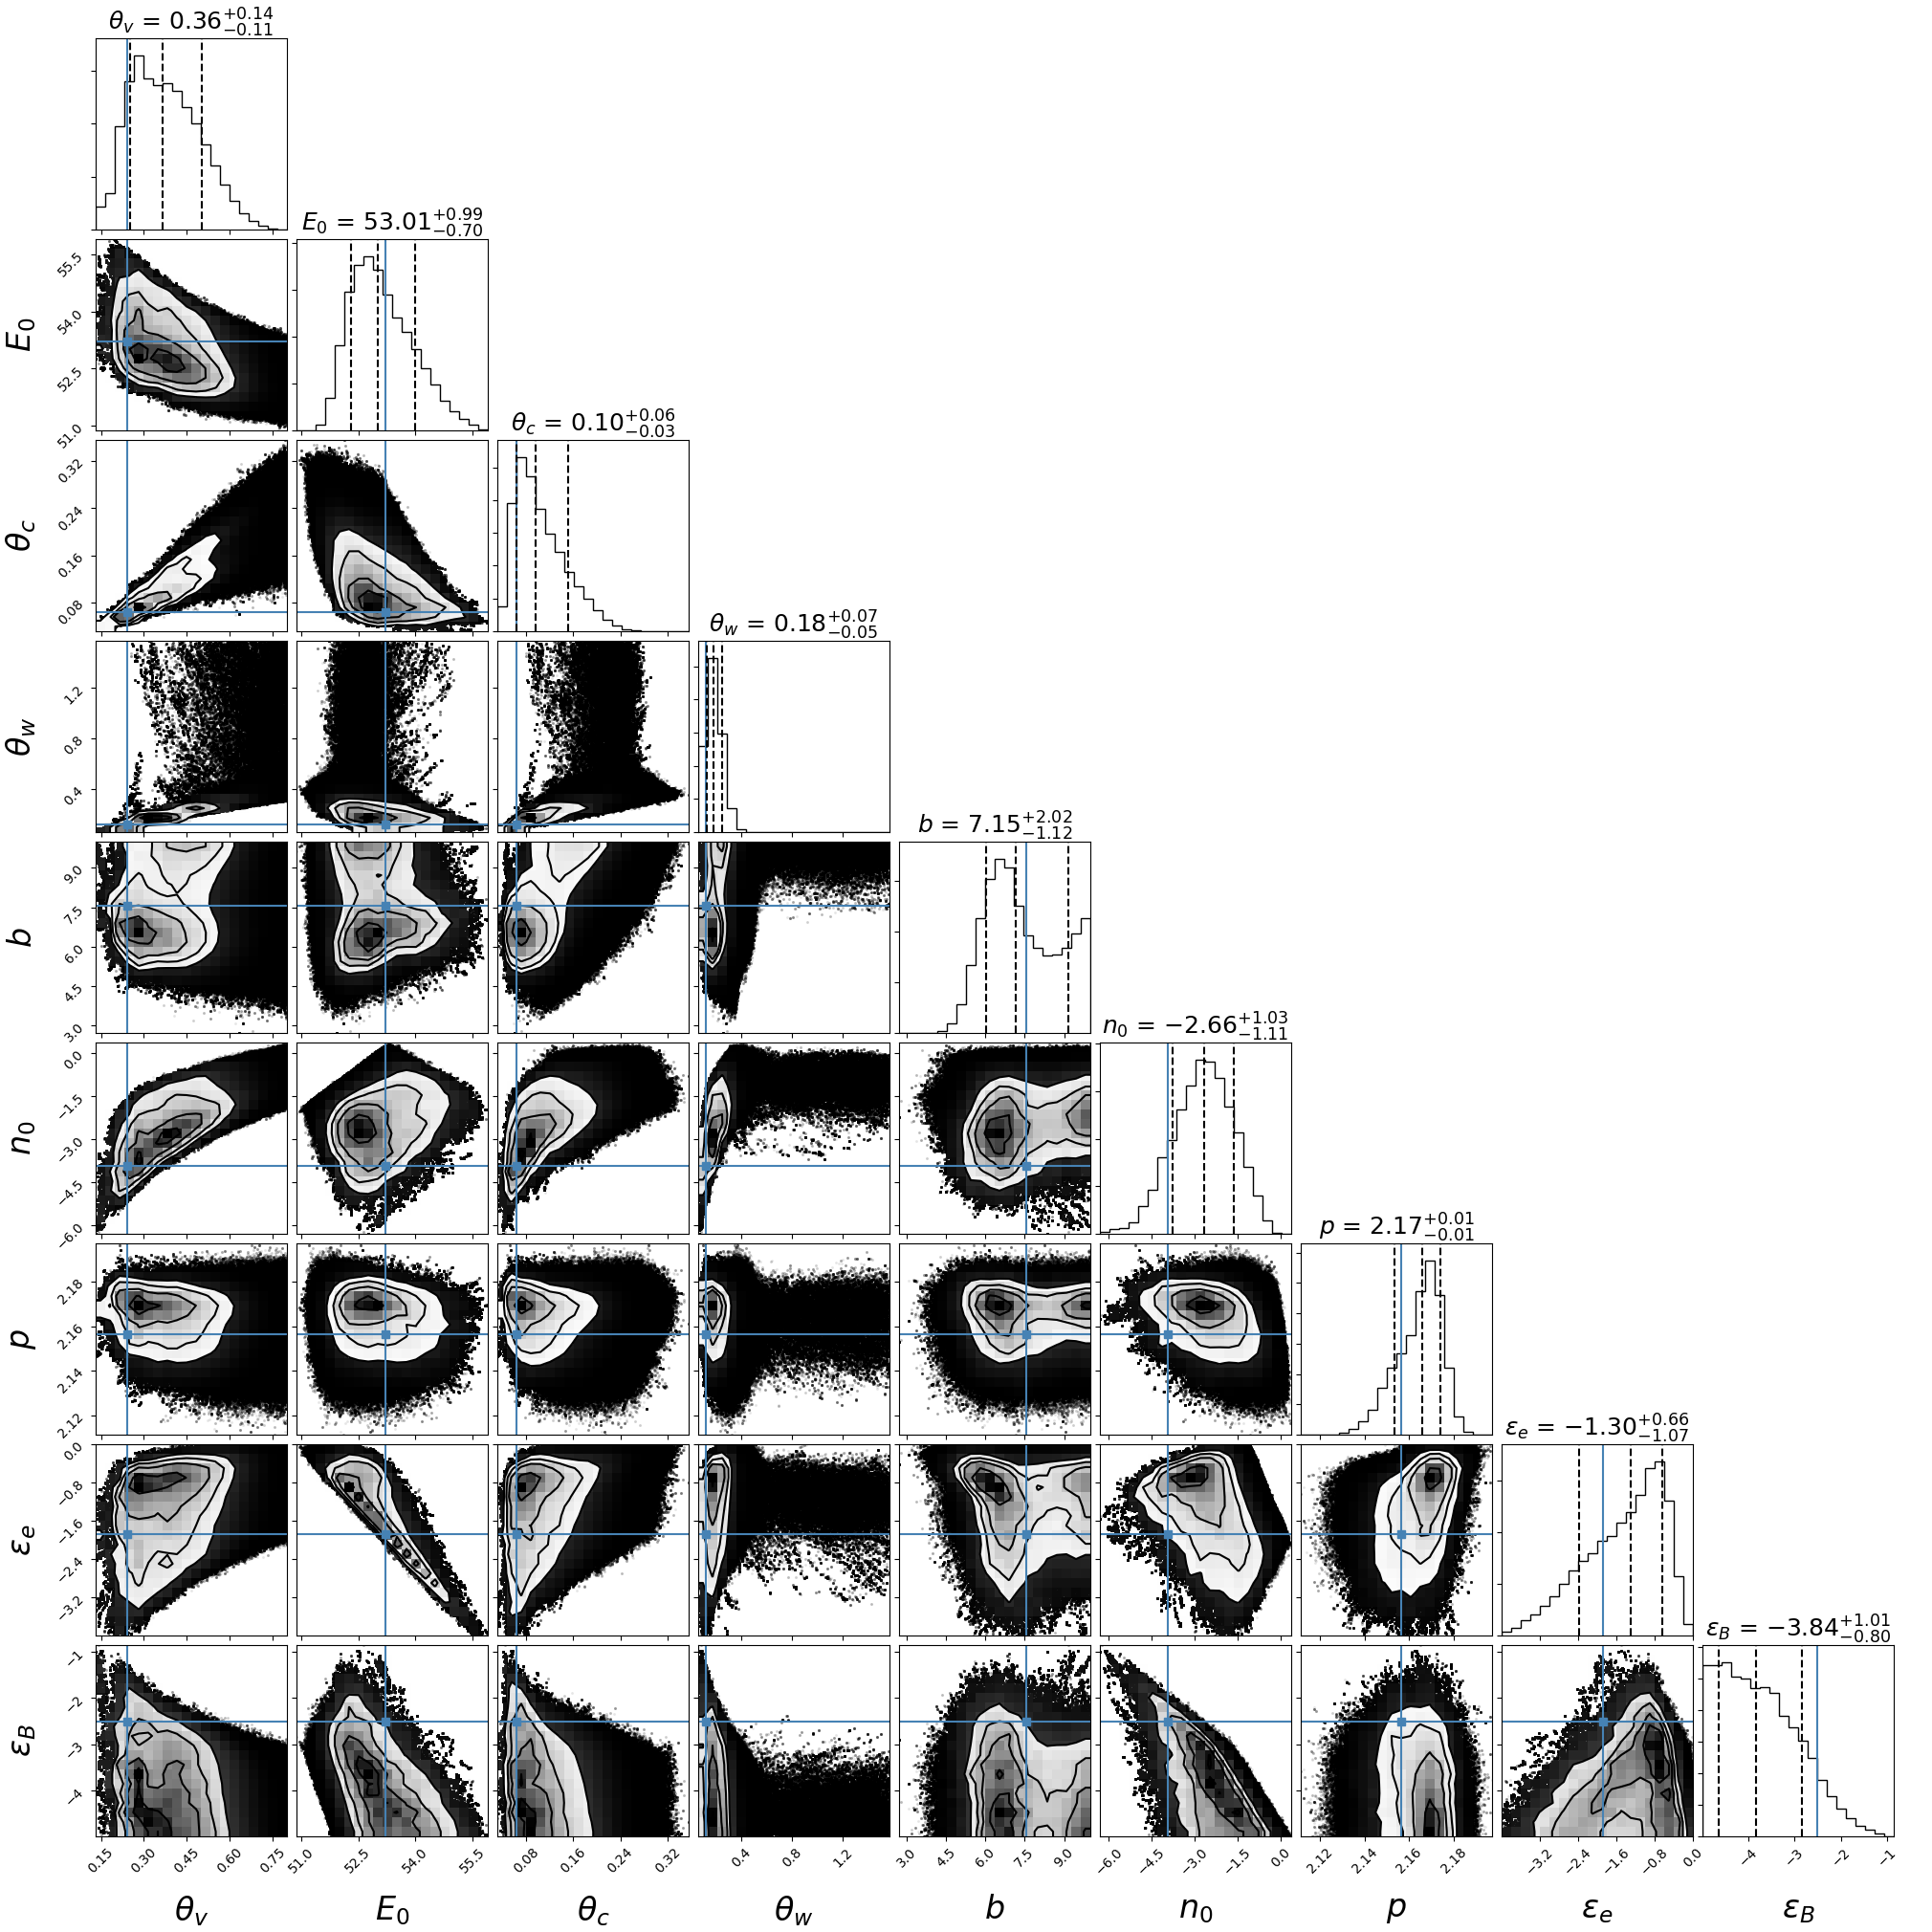
\includegraphics[width=\textwidth]{figs/cornerPowerlaw.png}
	\caption{Views of the posterior parameter distribution for a power law jet fit to the \gwbns{} afterglow.  The diagonal contains one-dimensional marginalized posteriors for each fit parameter, while the off-diagonal plots contain two-dimensional maps of the posterior marginalized over all but the two corresponding parameters. \label{fig:cornerPowerlaw}}
\end{figure*}

Figures \ref{fig:cornerGaussian} and \ref{fig:cornerPowerlaw} show the one- and two-dimensional marginalized views of the posterior distribution for the Gaussian. and power law jet model fits, respectively.  Table \ref{tab:MCMC} additionally gives constraints on the total jet energy \Etot{} and the ratio $\thobs/\thC$. The parameters $E_0$, $n_0$, $\epse$, and $\epsB$ are only constrained to within an order of magnitude, due partially to the observed radio, optical, and x-ray data all lying on the same synchrotron power-law segment.  These parameters are shared between jet models, and are broadly consistent between the two fits with the possible exception of $n_0$.  The electron energy index $p$ is extremely well constrained by both models, of course, due precisely to the large range of data laying on the same synchrotron segment.  The total jet energy in both models in constrained to be on the order $10^{51}$erg.

Of most interest are the geometric parameters: the viewing angle $\thobs$ and the jet structure parameters $\thC$, $\thW$, and $b$.  Encouragingly, the fits agree with the back-of-the-envelope reasoning from the analytic closure relations and break time scalings.  Both models constrain $\thobs$ and $\thC$ reasonably well, but constrain the combination $\thobs/\thC$ far better.  This is very evident by the corresponding map of the posterior in Figures \ref{fig:cornerGaussian} and \ref{fig:cornerPowerlaw}, which clearly displays a preferred linear relationship between $\thobs$ and $\thC$.  This is the manifestation of the structured jet closure relations with $g \approx \geff(\thobs/\thC)$.  The looser constraint on $\thobs/\thC$ in the power law jet comes from the additional freedom of the $b$ parameter, which has an effect on $\geff$ in that model (see Equation \eqref{eq:geff}). The truncation angle $\thW$ is essentially unconstrained in the Gaussian fit as a far off-axis phase was not observed.  In the power law fit, however, $\thW$ is constrained to be quite narrow so as to avoid the early bright wings.

Despite the tight constraints each model gives on $\thobs$, $\thC$, and especially $\thobs/\thC$, the resulting posteriors are incompatible with each other.  The median and 68\% uncertainties in Table \ref{tab:MCMC} display only a mild tension in $\thobs$  and $\thC$ themselves, but a very large discrepancy in $\thobs/\thC$.  This is, of course, due to the very different energy profiles $E(\theta)$ in each model.  Both models can easily accommodate a rising light curve $F_\nu \sim t^{0.9}$, that is produce an effective structure parameter $\geff = 7.5$, but do so using very different geometries.  


%%%%%%%%%%%%%%%
%
%.  DISCUSSION
%
%%%%%%%%%%%%%%%

\section{Discussion}\label{sec:discussion}

\subsection{Inferring $\thobs$ and $E(\theta)$}

Information about the viewing angle and jet structure is clearly encoded within misaligned afterglow light curves, primarily through the temporal slope $\alpha$ during the structured phase.   This parameter alone, however, does not uniquely identify a particular structure model or observer inclination.  When trying to infer information about a particular afterglow, there is a massive degeneracy between $E(\theta)$ and $\thobs$.  

This degeneracy is a blessing and a curse.  The presence of an extended slowly decaying or rising afterglow is a largely model independent prediction of misaligned viewing and the presence of non-trivial jet structure.  Unfortunately, this same model independence makes it very difficult to distinguish between jet structure profiles, leaving both $E(\theta)$ and $\thobs$ uncertain.

\begin{figure}
	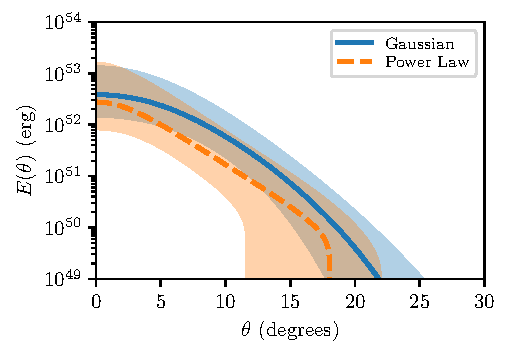
\includegraphics[width=\columnwidth]{figs/fit_E_theta.pdf}
	\caption{Inferred $E(\theta)$ for \gwbns{} assuming Gaussian (blue, solid line) or power law (orange, dashed line) structure models.  Lines show the median posterior value for $E(\theta)$ at each fixed value of $\theta$, shaded regions show the symmetric 68\% confidence interval (16\% and 84\% quantiles) at each $\theta$. \label{fig:fit_E_theta.pdf}}
\end{figure}

There are at least two ways of easing this degeneracy: incorporating data other than the afterglow light curve itself and looking at population-level statistics.  Utilizing posteriors from the gravitational wave signal or fitting the VLBI observations of superluminal apparent motion can greatly improve constraints on $\thobs$ \citep{Troja:2018aa, Hotokezaka:2018aa, Ghirlanda:2019aa}.  Since the afterglow presumably provides good constraints on $\geff$ (via $\alpha$), improved knowledge of $\thobs$ immediately improves knowledge of $\thC$, $b$, and any other parameters relevant to $E(\theta)$.  In some cases this may rule out a particular $E(\theta)$ entirely by pushing the relevant parameters to extreme values, for instance it is hard (but not impossible) to reconcile the observations of \gwbns{} with a power law jet with $b=2$.

\begin{figure}
	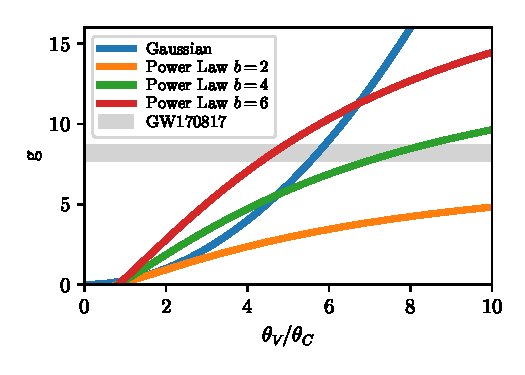
\includegraphics[width=\columnwidth]{figs/g_plot.pdf}
	\caption{Structure parameter $g$ as a function of $\thobs/\thC$ for different structured jet models: Gaussian (blue), $b=2$ power law (orange), $b=4$ power law (green), and $b=6$ power law (red).  The inferred value $g = 8.2\pm0.5$ for \gwbns{} is shown in as the grey band. \label{fig:gPop}}
\end{figure}

In the future, it may be possible to attack the question of determining $E(\theta)$ at the population level.  Figure \ref{fig:gPop} shows the structure parameter $g$ as a function of $\thobs/\thC$ for several jet models, as well as the inferred value from \gwbns{}.  If all short GRB jets share a jet profile shape, they should trace out a single curve in this space.  As more misaligned afterglows are observed, measurements of $g$ can populate this diagram and potentially rule out models (such as potentially the $b=2$ power law).  Model-independent constraints on $\thobs/\thC$ will greatly aid this procedure.  Moreover, each structure model should predict a different observed distribution of $g$, depending on the shape of the $g(\thobs/\thC)$ curve and the detectability of each burst.  With sufficient observations of $g$ alone and understanding of the observational biases, it may be possible to infer the underlying $g(\thobs/\thC)$ curve and $E(\theta)$ itself.

\subsection{Comparison With Other \gwbns{} Analyses}


Many groups have used structured jet models to analyze the afterglow of \gwbns{}, among the most recent with comparable models are \citet{Hotokezaka:2018aa, Ghirlanda:2019aa, Lamb:2019aa, Wu:2018aa}.  Of these, \citet{Hotokezaka:2018aa, Ghirlanda:2019aa, Lamb:2019aa} use semi-analytic methods similar to the present work to construct afterglow light curves, while \citet{Wu:2018aa} utilizes analytic scaling relations and a template bank constructed from numerical simulations.  Additionally, \citet{Hotokezaka:2018aa, Ghirlanda:2019aa} include constraints from the VLBI measurements of the \gwbns{} radio centroid's apparent superluminal motion.

TODO: INCLUDE BRIEF COMPARISON TO EACH.  NOTE DIFFERENT MODELS PRODUCE SAME LIGHT CURVE, STRONG EFFECT OF VLBI.

\subsection{O3 And Beyond}

In the coming years there will be more \gwbns{}-like events, although perhaps few with as extensive followup campaigns.  Since many of these events may be faint and distant, it will be important to leverage as much information from the afterglow light curve as possible.  As shown here, and evidenced by the diversity of models that have ``fit'' the \gwbns{} afterglow, there is a large degeneracy between viewing angle and jet structure profile.  To make robust inferences about these events, several flexible jet models must be included in the analysis.  

We hope \afterglowpy{} and similar products will aid these analyses in the future.  

\section{Summary}\label{sec:summary}

We have constructed flexible models for the electromagnetic afterglows of angularly structured relativistic jets.  Through analytic approximations we can identify the basic phases of the structured afterglow light curve, determining formulae for the characteristic break time scales and closure relations.  We find the closure relations depend on a single parameter we call $g$ relating to the jet structure and viewing angle.  Measurements of $g$ itself are model independent, but relating it back to physical parameters of the jet is not.

We also constructed a numerical model of the afterglows of structured jets, implemented in the public \python{} package \afterglowpy{}. \afterglowpy{} computes afterglow light curves on the fly utilizing semi-analytic approximations to the jet evolution and synchrotron emission, taking into account relativistic beaming, the equal time of arrival surface, jet angular structure, trans-relativistic evolution, and jet spreading.  It is fast enough to be incorporated in MCMC parameter estimation routines.  Fitting the \gwbns{} afterglow with multiple \afterglowpy{} models reveals the degeneracy between jet structure and viewing angle.

\newpage


\appendix
\section{Derivation of the Off-Axis Jet equations}\label{app:derive1}

  The \emph{structured jet} model is a generalization of the simple top hat jet where the energy and Lorentz factor vary with the polar angle.  The light curves of structured jets display more complex behavior than top hats, which we can understand through some simple analytic relationships.
  
  Firstly, the complex behavior of a structured jet is due to relativistic beaming enhancing the jet emission at different angles as a function of time.  Once the jet becomes non-relativistic this effect is suppressed and the entire jet comes into view.  As such we will focus on the emission when the jet remains relativistic, the late-time behavior is the same as any Newtonian jet of comparable total energy.  Numerical simulations and analytic considerations have demonstrated that jet spreading does not begin in earnest until the blast wave approaches sub relativistic velocity so we will also neglect the effects of spreading and assume each sector of the jet evolves independently.  Lastly, we will assume when each sector of the blast wave is visible it is in the deceleration regime.  In this phase of evolution the blast wave Lorentz factor evolves according to:
  \begin{equation}
	\gamma(t; \theta) \propto \sqrt{\frac{E(\theta)}{n_0}}\ t^{-3/2}\ . \label{eq:lorentzEvolution}
\end{equation}
  In the above $\gamma$ is the Lorentz factor of the shocked fluid at an angle $\theta$ from the jet axis at lab time (in the burster frame) $t$.  The blast wave expands into a medium of constant density $n_0$ and has an angularly dependent isotropic-equivalent energy $E(\theta)$.  The forward shock is at a position $R(t; \theta)$, and moves at a speed $\beta_s = (1-\gamma_s^{-2})^{1/2}$, where $\gamma_s^2 = 2 \gamma^2$ is the Lorentz factor of the shock.  Assuming $\gamma \gg 1$ gives:
\begin{equation}
	R(t; \theta) = ct\left(1-\frac{1}{16 \gamma^2(t; \theta)}\right)\ .
\end{equation}
We denote the angle between the viewer and a particular jet sector as $\psi$ and its cosine and $\mu = \cos \psi$.  Photons emitted at time from a sector of the blast wave at time $t$ will be seen by the observer at $\tobs$:
\begin{equation}
	\tobs = t - \frac{\mu}{c} R(t,\theta) = (1-\mu)t + \frac{\mu}{16}\frac{t}{ \gamma^2(t,\theta)} \label{eq:tobs}
\end{equation}

The observed flux depends on the luminosity distance $d_L$, viewing angle $\thobs$, and rest-frame emissivity $\varepsilon'_{\nu'}$.  The Doppler factor is $\delta = \gamma^{-1} (1-\beta\mu)^{-1}$, where $\beta=(1-\gamma^{-2})^{1/2}$ is the fluid three velocity.  The observed flux can then be expressed as a volume integral, where the integrand is evaluated at the time $t$ corresponding to $\tobs$ and position ${\bf r}$.
\begin{equation}
	F_\nu(\tobs, \nuobs) = \frac{1}{4\pi d_L^2} \int d^3{\bf r} \ \delta^2 \varepsilon'_{\nu'}\ .
\end{equation}  
The blast wave emits from a region of width $\Delta R \propto \delta_s \gamma_s \gamma^{-2} R $ where $\delta_s$ is the Doppler factor associated with the shock Lorentz factor $\gamma_s$. At a given observer time, the emission will be dominated by a region of (rest-frame) angular size $\Delta \Omega$.  The flux can then be approximated as:
\begin{equation}
	F_\nu(\tobs, \nuobs) \propto R^2 \Delta R \Delta \Omega \delta^2 \varepsilon'_{\nu'} \propto \Delta \Omega\ t^3 \gamma^{-2} \gamma_s \delta_s \delta^2 \varepsilon'_{\nu'}
\end{equation}.
The emissivity $\varepsilon'_{\nu'}$ depends on the fluid Lorentz factor, the frequency $\nuobs$, and numerous (constant) microphysical parameters.  We parameterize the dynamic dependence as $\varepsilon'_{\nu'} \propto \gamma^{s_1} t^{s_2} {\nu'}^\beta = t^{s_2} \gamma^{s_1}\delta^{-\beta} \nuobs^\beta$. The values of $s_1$, $s_2$, and $\beta$ in synchrotron regimes are given in Table \ref{tab:specSlopes}.  This leads to a flux of:
\begin{equation}
	F_\nu \propto \Delta \Omega\ t^{3+s_2} \gamma^{-1+s_1} \delta_s \delta^{2-\beta} \nuobs^\beta\ . \label{eq:fluxApprox}
\end{equation}

\begin{deluxetable}{CCCC}
	\tablecaption{Dependence of $\varepsilon'_{\nu'} \propto \gamma^{s_1} t^{s_2} \nu'^{\beta}$ in various spectral regimes. \label{tab:specSlopes}}
	\tablehead{\colhead{Regime}& \colhead{$s_1$} & \colhead{$s_2$} & \colhead{$\beta$}}
	\startdata
	\nu'<\nu'_m<\nu'_c     & 1 & 0 & 1/3 \\
	\nu'_m<\nu'<\nu'_c     & (3p+1)/2 & 0 & (1-p)/2 \\
	\nu'_m<\nu'_c<\nu'     & 3p/2 & -1 & -p/2 \\ 
	\hline 
	\nu' < \nu'_c < \nu'_m & 7/3 & 2/3 & 1/3 \\
	\nu'_c < \nu' < \nu'_m & 3/2 & -1 & -1/2 \\
	\nu'_c < \nu'_m < \nu' & 3p/2 & -1 & -p/2 \\ 
	\enddata
\end{deluxetable}
The Doppler factor depends on the fluid Lorentz factor and whether the material is on-axis. The on/off axis boundary occurs at $\gamma^{-1} \approx \sin \psi$ (ie. $\beta \approx \mu$).  One can write:
\begin{equation}
	\delta = \left \{ \begin{matrix}
				\frac{1}{2} \gamma^{-1} \sin^{-2}\psi/2,  & \text{if } \gamma \gg 1 \text{ and } \sin{\psi} \gg \gamma^{-1} \ \ \text{(off-axis)} \\
				2 \gamma, & \text{if } \gamma \gg 1 \text{ and } \sin{\psi} \ll \gamma^{-1} \ \  \text{(on-axis)} \\
				1  & \text{if } \beta \ll 1\ \  \text{(non-relativistic)} \\ \end{matrix} \right . \ .
\end{equation}
The observer time can be similarly simplified in both limits:
\begin{equation}
	\tobs = \left \{ \begin{matrix}
				\frac{1}{2} \psi^2 t,  & \text{if }\sin{\psi} \gg \gamma^{-1}\ \ \text{(off-axis)} \\
				\frac{1}{16} \gamma^{-2} t, & \text{if } \sin{\psi} \ll \gamma^{-1} \ \  \text{(on-axis)} \end{matrix} \right . \ .
\end{equation}
As can the flux:
\begin{equation}
	F_\nu \propto \left \{ \begin{matrix}
				\Delta \Omega t^{3+s_2} \gamma^{-4+s_1+\beta} \psi^{-6+2\beta}\nuobs^\beta,  & \text{(off-axis)} \\
				\Delta \Omega t^{3+s_2} \gamma^{2+s_1-\beta} \nuobs^\beta, & \text{(on-axis)} \end{matrix} \right . \ .
\end{equation}
The behavior of the Doppler factor informs the scaling of $\Delta \Omega$.  If any part of the jet is on-axis, its emission is enhanced by $\sim \gamma^2$ over the off-axis material and will dominate.  An observer for whom the entire jet is off-axis must be situated at some large $\thobs$, outside the outermost jet material.  At early times the entire jet will be beamed off-axis, with emission from the near edge (with the smallest $\psi$ and presumably $\gamma$) contributing most to the emission.  The absence of any particular angular scale in this regime indicates $\Delta \Omega$ will be roughly constant.  For an on-axis observer $\Delta \Omega \sim \sin^2 \psi_{\rm{max}} \propto \gamma^{-2}$ until the entire jet is on-axis, at which point $\Delta \Omega$ is again constant.  Hence:
\begin{equation}
	F_\nu \propto \left \{ \begin{matrix}
				t^{3+s_2} \gamma^{-4+s_1+\beta} \psi^{-6+2\beta}\nuobs^\beta,  & \text{(off-axis)} \\
				t^{3+s_2} \gamma^{s_1-\beta} \nuobs^\beta, &  \text{(on-axis, pre jet break)} \\
				t^{3+s_2} \gamma^{2+s_1-\beta} \nuobs^\beta, & \text{(on-axis, post jet break)} \end{matrix} \right . \ .
\end{equation}
Finally, for off-axis emission $t \propto \tobs$ and hence $\gamma \propto \tobs^{-3/2}$.  For on-axis observers $\tobs \propto \gamma{-2} t \propto t^4$, hence $t\propto \tobs^{1/4}$ and $\gamma \propto \tobs^{-3/8}$. Giving finally:
\begin{equation}
	F_\nu \propto \left \{ \begin{matrix}
				\tobs^{9+s_2 -3(s_1+\beta)/2} \psi^{-6+2\beta}\nuobs^\beta,  & \text{(off-axis)} \\
				\tobs^{(3+s_2)/4+3(-s_1+\beta)/8} \nuobs^\beta, &\text{(on-axis, pre jet break)} \\
				\tobs^{s_2/4 + 3(-s_1+\beta)/8} \nuobs^\beta, & \text{(on-axis, post jet break)} \end{matrix} \right . \ .
\end{equation}
These formulae capture the standard behavior of top-hat jets, as well as any jet that is \emph{fully} on-axis or off-axis.  What they fail to (easily) demonstrate is the behavior of a structured jet which transitions continuously from one state to the other over the course of observation.

\section{Derivation of the Structured Jet equations}\label{app:derive2}

A jet with a non-trivial angular distribution of energy can exhibit qualitatively different behaviour than a simple top hat, particularly when observed at a significant viewing angle.  While the initial off-axis and final on-axis post jet-break evolutions are identical, these are separated by a transition phase where the sector dominating the emission scans over the jet surface.  This transition phase begins at the end of the off-axis phase: when a sector of the jet first decelerates to include the observer in its beaming cone.  This will necessarily be from the wings/edge of the jet, the material with the lowest Lorentz factor and smallest angle $\psi$ to the observer.  As the blastwave decelerates more energetic material from nearer the core will come into view and the high latitude emission will dim.  Finally the core of the jet ($\theta = 0$ or $\psi = \thobs$) decelerates and becomes visible to the observer.  At this point the entire jet is on-axis and evolution continues as in the post jet-break phase.

At each moment during the structure phase the emission is dominated by material that just came on-axis, where $\gamma^{-1} = \sin \psi$.  To find the overall behaviour we first determine $\tobs(\psi)$ and $F_\nu(\psi)$ for material whose emission is peaking (coming on-axis).  Since the structure phase occurs when motion is still relativistic, we can assume $\gamma \gg 1$ and hence $\sin \psi \ll 1$.  In this approximation:
\begin{eqnarray}
	\mu \approx 1 - \frac{1}{2}\sin^2\psi \ , \label{eq:muPsi}\\
	\delta_s \approx \delta \approx \gamma = \csc \psi\ . \label{eq:deltaPsi}
\end{eqnarray}
The material dominating the emission is in the plane between the observer and the jet axis, denoted by $\phi = 0$. Along this line we have $\psi = \thobs - \theta$, and can use $\psi$ or $\theta$ interchangeably to denote latitude.  From Equation \eqref{eq:lorentzEvolution} we have $t\propto E(\theta)^{1/3} \gamma^{-2/3}$.  Using Equation \eqref{eq:tobs} and \eqref{eq:muPsi} we find that material at $\psi$ will come on-axis at observer time:
\begin{equation}
	\tobs(\psi) = \frac{9}{16} t \sin^2\psi  \propto E(\theta)^{1/3} \sin^{8/3} \psi\ . \label{eq:tobsPsi}
\end{equation}
The peak flux from material at $\psi$ can be determined from Equation \eqref{eq:fluxApprox}.  Using Equation \eqref{eq:deltaPsi} and taking $\Delta \Omega \propto \gamma^{-s_3}$ gives an observed flux:
\begin{equation}
	F_\nu(\psi) \propto t^{3+s_2} \gamma^{2+s_1-s_3-\beta} \nuobs^\beta \propto E(\theta)^{1+s_2/3} (\sin \psi)^{-s_1 + 2 s_2/3 +s_3+\beta} \nuobs^\beta  \ . \label{eq:FnuPsi}
\end{equation}
	Equations \eqref{eq:tobsPsi} and \eqref{eq:FnuPsi} describe the evolution of the flux in the structure phase in terms of the parameter $\psi$, which varies from $\mathrm{min} (0, \thobs-\thW)$ to $\thobs$.  In principle one would like to invert Equation \eqref{eq:tobsPsi} and substitute into Equation \eqref{eq:FnuPsi} to obtain $F_\nu(\tobs)$ itself.  Unfortunately, in general this is impossible to do in closed form because $E(\theta)$ is non-trivial. 
	
	We can obtain the temporal power law slope of the light curve by differentiating both Equations \eqref{eq:tobsPsi} and \eqref{eq:FnuPsi} with respect to $\psi$.  Noting that $dE/d\psi = -dE/d\theta$ we obtain for the individual derivatives:
\begin{eqnarray}
	\frac{d \log \tobs}{d \psi} = \frac{8}{3} \cot \psi - \frac{1}{3} \frac{d \log E}{d \theta}\ , \\
	\frac{d \log F_\nu}{d \psi} = \left(-s_1 + \frac{2}{3} s_2 +s_3+\beta\right)\cot \psi - \left(1+\frac{1}{3}s_2\right) \frac{d \log E}{d \theta}\ .
\end{eqnarray}
Taking the ratio and simplifying gives:
\begin{eqnarray}
	\frac{d \log F_\nu}{d \log \tobs}(\psi) = \frac{3 \beta - 3s_1 + 2s_2+3s_3 + (3+s_2)g(\psi)}{ 8+g(\psi)} \\
	g(\psi) \equiv -\tan \psi \frac{d \log E}{d \theta}\ .
\end{eqnarray}
The parameter $g$ is directly measurable from the light curve, given the spectral information which fixes $\beta$, $s_1$, and $s_2$.

The full flux scaling equations also require an updated energy and circumburst density scaling. We can obtain the scalings for energy and density from dimensional analysis, following \cite{van-Eerten:2012ac} (specifically, by making use of the fact that the overall flux scalings for the different spectral regimes should obey those presented in table 1 of that paper).

{\color{red}[RED STUFF IS WRONG SOMEHOW]
  For energy, it follows that (below $\nu_c$)
\begin{equation}
	\frac{d \log F}{d \log E} = \frac{d \log F}{d \Psi} \frac{d \Psi}{d \log E} = - \frac{d \log F}{d \Psi} \frac{d \theta}{d \log E} = \left(s_1 - \frac{2}{3} s_2 - s_3 -\beta\right) h(\Psi) + 1 + \frac{1}{3} s_2,
\end{equation}
where
\begin{equation}
	h(\Psi) \equiv \cot \Psi \frac{d \log E}{d \theta}.
\end{equation}
For the density $n_0$ we have (below $\nu_c$)
\begin{equation}
	\frac{d \log F}{d \log n_0} = \frac{2+s_3}{8}
\end{equation}
}
Altogether, we obtain
\begin{eqnarray}
F_D & \propto & (1+z)^{(38-5g(\Psi)-9s_3)/3(8+g(\Psi))} \epsilon_e^{-2/3} \epsilon_B^{1/3} n_0^{(6+4g+3s_3)/3(8+g(\Psi))} E_0^{(26-3s_3)/3(8+g(\Psi))} t_{obs}^{(-2+3s_3+3g(\Psi))/(8+g(\Psi))} \nu^{1/3} \nonumber \\
F_E & \propto & (1+z)^{(46-7g(\Psi)-9s_3)/3(8+g(\Psi))} \epsilon_B^{1} n_0^{(14+6g(\Psi)+3s_3)/3(8+g(\Psi))} E_0^{(34-3s_3)/3(8+g(\Psi))} t_{obs}^{(-14+9s_3+11g(\Psi))/3(8+g(\Psi))} \nu^{1/3} \nonumber \\
F_F & \propto & (1+z)^{(24-3g(\Psi)-6s_3)/2(8+g(\Psi))} \epsilon_B^{-1/4} n_0^{(-8+3g(\Psi)+4s_3)/4(8+g(\Psi))} E_0^{(8-s_3)/(8+g(\Psi))} t_{obs}^{(-8+3s_3+2g(\Psi))/(8+g(\Psi))} \nu^{-1/2} \nonumber \\
F_G & \propto & (1+z)^{\frac{(-pg(\Psi)-3g(\Psi)+4p-6s_3+24)}{2(8+g(\Psi))}} \epsilon_e^{p-1} \epsilon_B^{(1+p)/4} n_0^{(g(\Psi)p + 5 g(\Psi) + 4s_3 + 8)/4(8+g(\Psi))} E_0^{(8+2p-s_3)/(8+g(\Psi))} t_{obs}^{3(-2p+s_3+g(\Psi))/(8+g(\Psi))} \nu^{(1-p)/2} \nonumber \\
F_H & \propto & (1+z)^{\frac{(-pg(\Psi)-2g(\Psi)+4p-6s_3+20)}{2(8+g(\Psi))}} \epsilon_e^{p-1} \epsilon_B^{(p-2)/4} n_0^{(g(\Psi)p+2g(\Psi)+4s_3-8)/4(8+g(\Psi))} E_0^{(6+2p-s_3)/(8+g)} t_{obs}^{(-6p-2+3s_3+2g(\Psi))/(8+g(\Psi))} \nu^{-p/2} \nonumber \\
\nu_m & \propto & (1+z)^{\frac{4-g(\Psi)}{8+g(\Psi)}} \epsilon_e^2 \epsilon_B^{1/2} n_0^{g(\Psi)/(16+2g(\Psi))} E_0^{4/(8+g(\Psi))} t_{obs}^{-12/(8+g(\Psi))} \nonumber \\
\nu_c & \propto & (1+z)^{\frac{-4+g(\Psi)}{8+g(\Psi)}} \epsilon_B^{-3/2} n_0^{-(3g(\Psi)+16)/2(8+g(\Psi))} E_0^{-4/(8+g(\Psi))} t_{obs}^{-2(2+g(\Psi))/(8+g(\Psi))} \nonumber \\
F_{peak} & \propto & (1+z)^{\frac{14-2g(\Psi)-3s_3}{8+g(\Psi)}} \epsilon_B^{1/2} n_0^{(4+3g(\Psi)+2s_3)/2(8+g(\Psi))} E_0^{(10-s_3)/(8+g(\Psi))} t_{obs}^{3(-2+s_3+g(\Psi))/(8+g(\Psi))}
\end{eqnarray}

\section{Shock Jump Conditions and Synchrotron Parameters}
\label{sec:shockJump}

Table \ref{tab:shockSync} lists the necessary quantities for calculating synchrotron emission from a forward shock.  Asymptotic expressions are given in the ultra-relativistic and non-relativistic limits.  The synchrotron emissivity in the fluid rest frame is:
\begin{equation}
	\varepsilon'_{\nu'} = \varepsilon_P \times \left \{ \begin{matrix}
											\left(\nu' / \nu_m\right)^{1/3} & \text{if } \nu' < \nu_m < \nu_c \\
											\left(\nu' / \nu_m\right)^{(1-p)/2} & \text{if } \nu_m < \nu'  < \nu_c \\
											\left(\nu_c/\nu_m\right)^{(1-p)/2}\left(\nu' / \nu_c\right)^{-p/2} & \text{if }\nu_m < \nu_c < \nu'\\
											\left(\nu' / \nu_c\right)^{1/3} & \text{if } \nu' < \nu_c < \nu_m \\
											\left(\nu' / \nu_c\right)^{-1/2} & \text{if } \nu_c <\nu' <  \nu_m \\
											\left(\nu_m / \nu_c\right)^{-1/2}\left(\nu' / \nu_m\right)^{-p/2} & \text{if } \nu_c < \nu_m < \nu'
											\end{matrix} \right .
\end{equation}


\begin{deluxetable}{CC|CCC}
\tablehead{ & \colhead{Expression} & \colhead{Coefficient} & \colhead{$ u \gg 1$} & \colhead{$ u \ll 1$}}
\tablecaption{Emission parameters at forward shock. \label{tab:shockSync}}
\startdata
n & 4 \gamma n_0 & 4 n_0 & \gamma & 1 \\
e & (\gamma-1)n \Mp c^2 & 4 \Mp c^2 n_0 &  \gamma^2 & \frac{1}{2} \beta^2 \\
B & \sqrt{8\pi e \epsB} & 4(2 \pi)^{1/2}(\Mp c^2)^{1/2} n_0^{1/2} \epsB^{1/2} & \gamma & 2^{-1/2} \beta \\ 
\hline
\gamma_m &  \frac{\epseb e}{n \Me c^2} & \frac{\Mp}{\Me} \epseb &  \gamma & \frac{1}{2} \beta^2 \\
\gamma_c & \frac{3 \Me c \gamma}{4 \sigT \epsB e t} & \frac{3}{16} \frac{\Me}{\Mp\sigT c}n_0 ^{-1} \epsB^{-1} & \gamma^{-1} t^{-1} & 2 \beta^{-2} t^{-1} \\
\varepsilon_P & \frac{\sqrt{3}}{2}\frac{\qe^3}{\Me c^2}(p-1)n B & 8 (6\pi)^{1/2} \frac{\Mp^{1/2} \qe^3}{\Me c} (p-1) n_0^{3/2} \epsB^{1/2} & \gamma^2 & 2^{-1/2} \beta \\ 
\nu_m & \frac{3}{4\pi}\frac{\qe}{\Me c} \gamma_m^2 B & 6 (2\pi)^{-1/2} \frac{\Mp^{5/2} \qe}{\Me^3} n_0^{1/2} \epseb^2 \epsB^{1/2} & \gamma^3 & 2^{-5/2} \beta^5 \\
\nu_c & \frac{3}{4\pi}\frac{\qe}{\Me c} \gamma_c^2 B & \frac{27}{128} (2\pi)^{-1/2} \frac{\Me \qe}{\Mp^{3/2}\sigT^2 c^2} n_0^{-3/2}  \epsB^{-3/2} & \gamma^{-1}t^{-2} & 2^{3/2}\beta^{-3}t^{-2} \\
\hline
E & \frac{4\pi}{9} \rho_0 c^2 R^3(4u^2+3)\beta^2 & \frac{16\pi}{9}\rho_0 c^2 & R^3 \gamma^2 & \frac{3}{4} R^3 \beta^2 \\
\beta_s & \frac{4 u \gamma}{4u^2+3} & 1 & 1 & \frac{4}{3}\beta 
\enddata
\end{deluxetable}


\bibliography{structuredJets_sources}


\end{document}
